\chapter{Minimization of Finite Automata}\label{ch-3}

We have seen that there are many different automata that can be
used to represent a given language. We would like to be able to
find an automaton for a language $L$ that is \emph{minimal}, that is, a
machine which can represent that language which has the fewest
number of states possible.

Finding such an optimal DFA will involve transforming a given
automaton into the most efficient equivalent machine. To effectively
accomplish this transformation, we must have a set of clear,
unequivocal directions specifying how to proceed. A \emph{\Index{procedure}}
is a finite set of instructions that unambiguously defines deterministic,
discrete steps for performing some task. As anyone who has programmed
a computer knows, it is possible to generate procedures that will
never halt for some inputs (or perhaps for \emph{all} inputs if the program
is seriously flawed). An \emph{\Index{algorithm}} is a procedure that is
guaranteed to halt on all (legal) inputs. In this chapter we will specify a
procedure for finding a minimal machine and then justify that this
procedure is actually an algorithm. Thus, the theorems and definitions
will show how to transform an inefficient DFA into an optimal
automaton in a straightforward manner that can be easily programmed.

%3.1 HOMOMORPHISMS AND ISOMORPHISMS
\section{Homomorphisms and Isomorphisms}\label{sec-3.1}

One of our goals for this chapter can be stated as follows: Given
a language $L$, we wish to survey \emph{all} the machines that recognize
$L$ and choose the machine (or machines) that is ``smallest.'' It
will be seen that there is indeed a \emph{unique} smallest machine: $A_{R_L}$.
The automaton $A_{R_L}$ will be unique in the sense that any other
optimal DFA looks exactly like $A_{R_L}$ except for a trivial relabeling
of the state names.  The concept of two automata ``looking alike''
will have to be formalized to provide a basis for our rigorous
statements. Machines that ``look alike'' will be called \emph{isomorphic},
and the relabeling specification will be called an \emph{isomorphism}.\index{isomorphism!between DFAs}

We have already learned some facts about $A_{R_L}$, which stem from
the proof of Nerode's theorem. These are summarized below and show
that $A_{R_L}$ is indeed one of the optimal machines for the language $L$.

% Corollary 3.1
\begin{cor}\label{cor-3.1}
For any FAD language $L$, $L(A_{R_L}) = L$.

\emph{Proof.} This was shown when $(3) \Rightarrow (1)$ in Theorem \ref{thm-2.2} was
proved.
\end{cor}

Also, in the proof of $(1) \Rightarrow (2)$ in Nerode's theorem, the relation
$R^M$ (defined by a given DFA $M= \langle\Sigma,S,s_0,\delta,F\rangle$ for which $L(M)=L$)
was used to show $\|S\| \geq rk(R^M)$. Furthermore, in $(2) \Rightarrow (3)$,
right congruences such as $R^M$ that satisfied property $(2)$ must be
refinements of $R_L$, and so $rk(R^M) \geq rk(R_L)$. Thus
$\|S\| \geq rk(R^M) \geq rk(R_L) = \|S_{R_L}\|$, which leads immediately to the
following corollary.

% Corollary 3.2
\begin{cor}\label{cor-3.2}\index{finite automaton!minimal deterministic}
For any FAD language $L$, $A_{R_L}$ is a minimal deterministic finite automaton
that accepts $L$.

\emph{Proof.} The proof follows from the definition of a minimal DFA (Definition
\ref{dfn-2.7}); that is, if $M =\langle\Sigma,S,s_0,\delta,F\rangle$ is any machine that also
accepts $L$, then $\|S\| \geq \|S_{R_L}\|$.
\end{cor}

Besides being in some sense ``the simplest,'' the minimal machine has some
other nice properties. For example, if $A$ is minimal, then the right congruence
generated by $A$ is identical to the right congruence generated by the language
recognized by $A$; that is, $R^A = R_{L(A)}$ (see the exercises). Examples 3.1
and 3.2 illustrate the two basic ways a DFA can have superfluous states.

% Definition 3.1
\begin{dfn}\label{dfn-3.1}\index{accessible state}\index{connected DFA}
A state $s$ in a finite automaton $A =\langle\Sigma,S,s_0,\delta,F\rangle$ is called
\emph{accessible} iff
\[ \exists x_s \in \Sigma^* \ni \DBAR(s_0,x_s) = s \]
The automaton $A$ is called \emph{connected} iff
$$ (\forall s \in S)(\exists x_s \in \Sigma^*)(\DBAR(s_0,x_s)=s) $$
\end{dfn}

That is, a connected machine requires all states to be accessible; every state
$s$ of $S$ must be ``reachable'' from $s_0$ by some string $(x_s)$ in $\Sigma^*$
(different states will require different strings, and hence it is convenient to
associate an appropriate string $x_s$, with the state $s$). States that are not
accessible are sometimes called \emph{disconnected},\index{inaccessible state}\index{unreachable state}\index{disconnected DFA}
\emph{\Index{inaccessible}}, or \emph{unreachable}.

\subsection*{Example 3.1}

The machine defined in Figure \ref{fig-3.1} satisfies the definition of a deterministic
finite automaton, but is disconnected since $r$ cannot be reached by any string
from the start state $q$. Note that $x_q$ could be $\lambda$ or $\pmb{10}$, while
$x_t$ might be $\pmb{0}$ or $\pmb{111}$. There is no candidate for $x_r$.
Furthermore, $r$ could be ``thrown away'' without affecting the language that
this machine accepts. This will be one of the techniques we will use to minimize
finite automata: removing the inaccessible states.

There is a second way for an automaton to have superfluous states, as shown
by the automata in the following examples. An overabundance of states may be
present, recording nonessential information and consequently distinguishing
between strings in ways that are unnecessary.

% Figure 3.1
\begin{figure}
\centerline{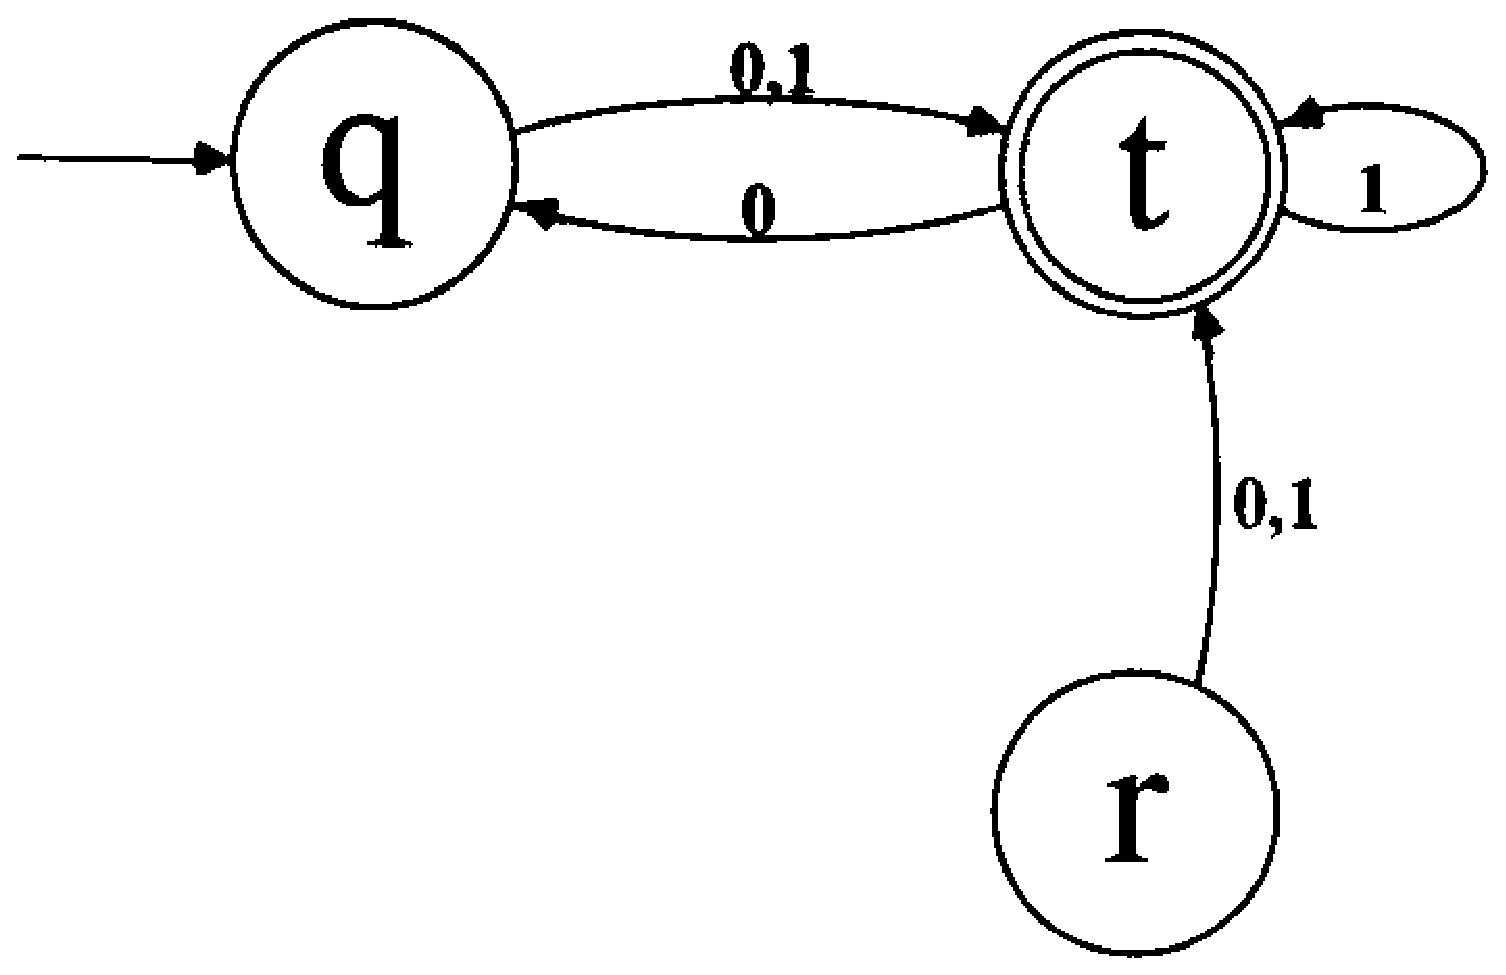
\epsfig{figure=ToFAfigures/fig3-1.eps,width=3in}}
\caption{The automaton discussed in Example 3.1}\label{fig-3.1}
\end{figure}

\subsection*{Example 3.2}

Consider the four-state DFA over $\{\pmb{a},\pmb{b}\}$ in which $s_0$ is the start and
only final state, defined in Figure \ref{fig-3.2}. This automaton is clearly connected,
but it is still not optimal. This machine accepts all strings whose length is a
multiple of 3, and $s_1$ and $s_2$ are really ``remembering'' the same
information, that is, that we currently have read a string that is one more than
a multiple of 3. The fact that some strings that end in $\pmb a$ are sent to $s_1$,
while those that end in $\pmb b$ may be sent to $s_2$, is of no real importance; we
do not have to ``remember'' what the last letter in the string actually was in
order to correctly accept the given language. The states $s_1$ and $s_2$ are in
some sense \emph{equivalent}\index{equivalent!DFA states}, since they are performing the same
function. The careful reader may have noticed that this language could have been
recognized with a three-state machine, in which a single state combines the
functions of $s_1$ and $s_2$.

Now consider the automaton shown in Figure \ref{fig-3.3}, in which there are three
superfluous states. This automaton accepts the same language as the DFA in
Figure \ref{fig-3.2}, but this time not only are $s_1$ and $s_2$ performing the same
function, but $s_3$ and $s_4$ are ``equivalent,'' and $s_0$ and $s_5$ are both
``remembering'' that there has been a multiple of three letters seen so far.
Note that it is not enough to check that $s_1$ and $s_2$ take you to exactly the
same places (as was the case in the first example); in this example, the arrows
coming out of $s_1$ and $s_2$ do \emph{not} point to the same places. The
important thing is that, when leaving $s_1$ or $s_2$, when $\pmb a$ is seen, we go to
\emph{equivalent} states, and when processing $\pmb b$ from $s_1$ or $s_2$,
we also go to \emph{equivalent} states. However, deciding whether two states are
equivalent or not is perhaps a little less straightforward than it may at first
seem. This sets the stage for the appropriate definition of equivalence.

% Figure 3.2
\begin{figure}
\centerline{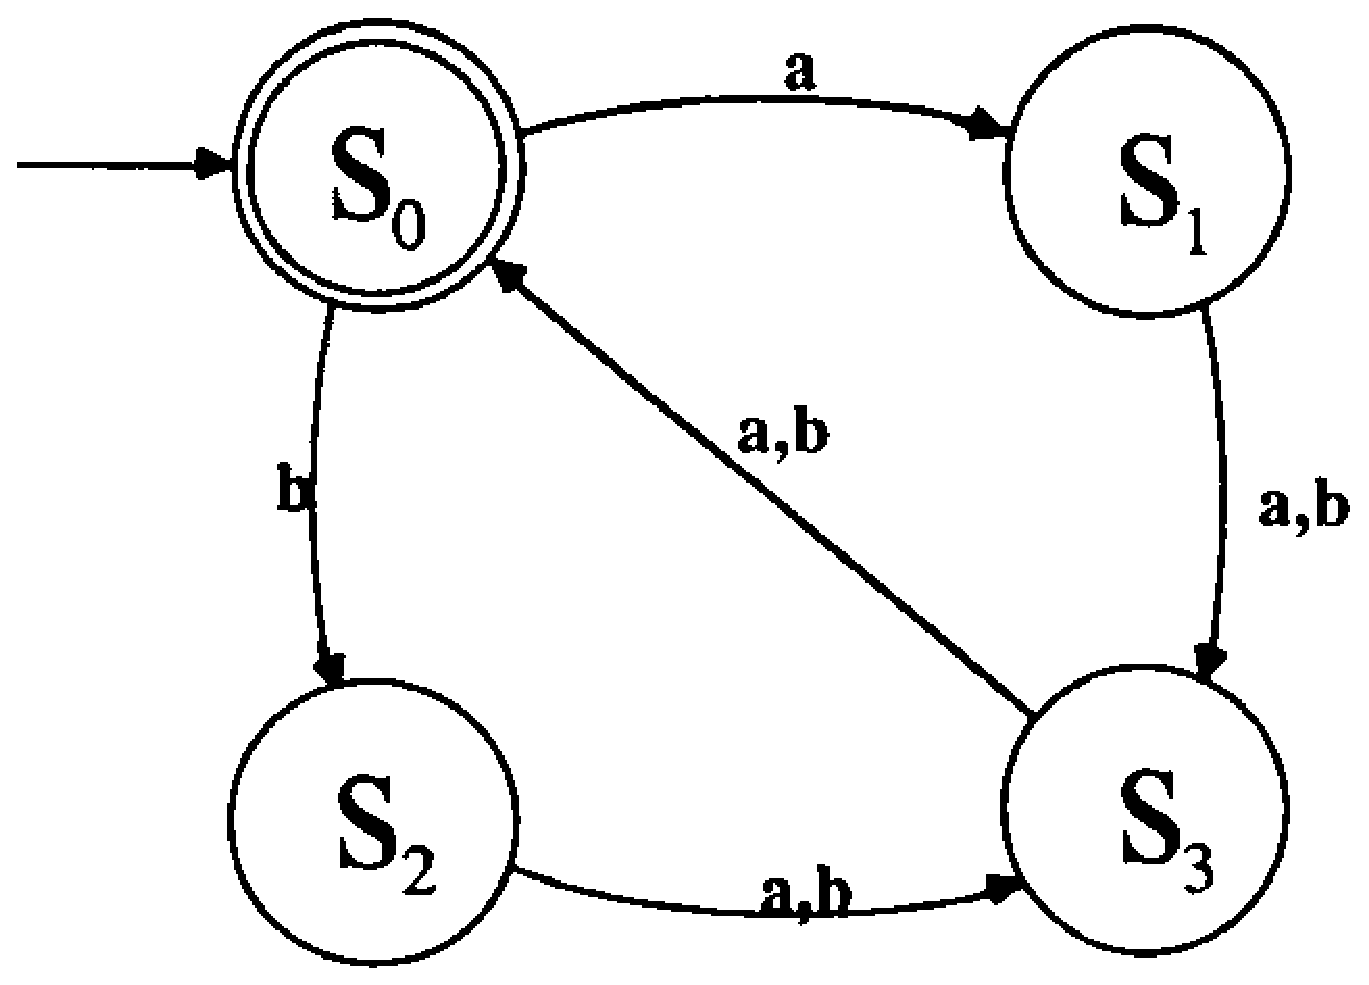
\epsfig{figure=ToFAfigures/fig3-2.eps,width=2.8in}}
\caption{The first automaton discussed in Example 3.2}\label{fig-3.2}
\end{figure}

% Figure 3.3
\begin{figure}
\centerline{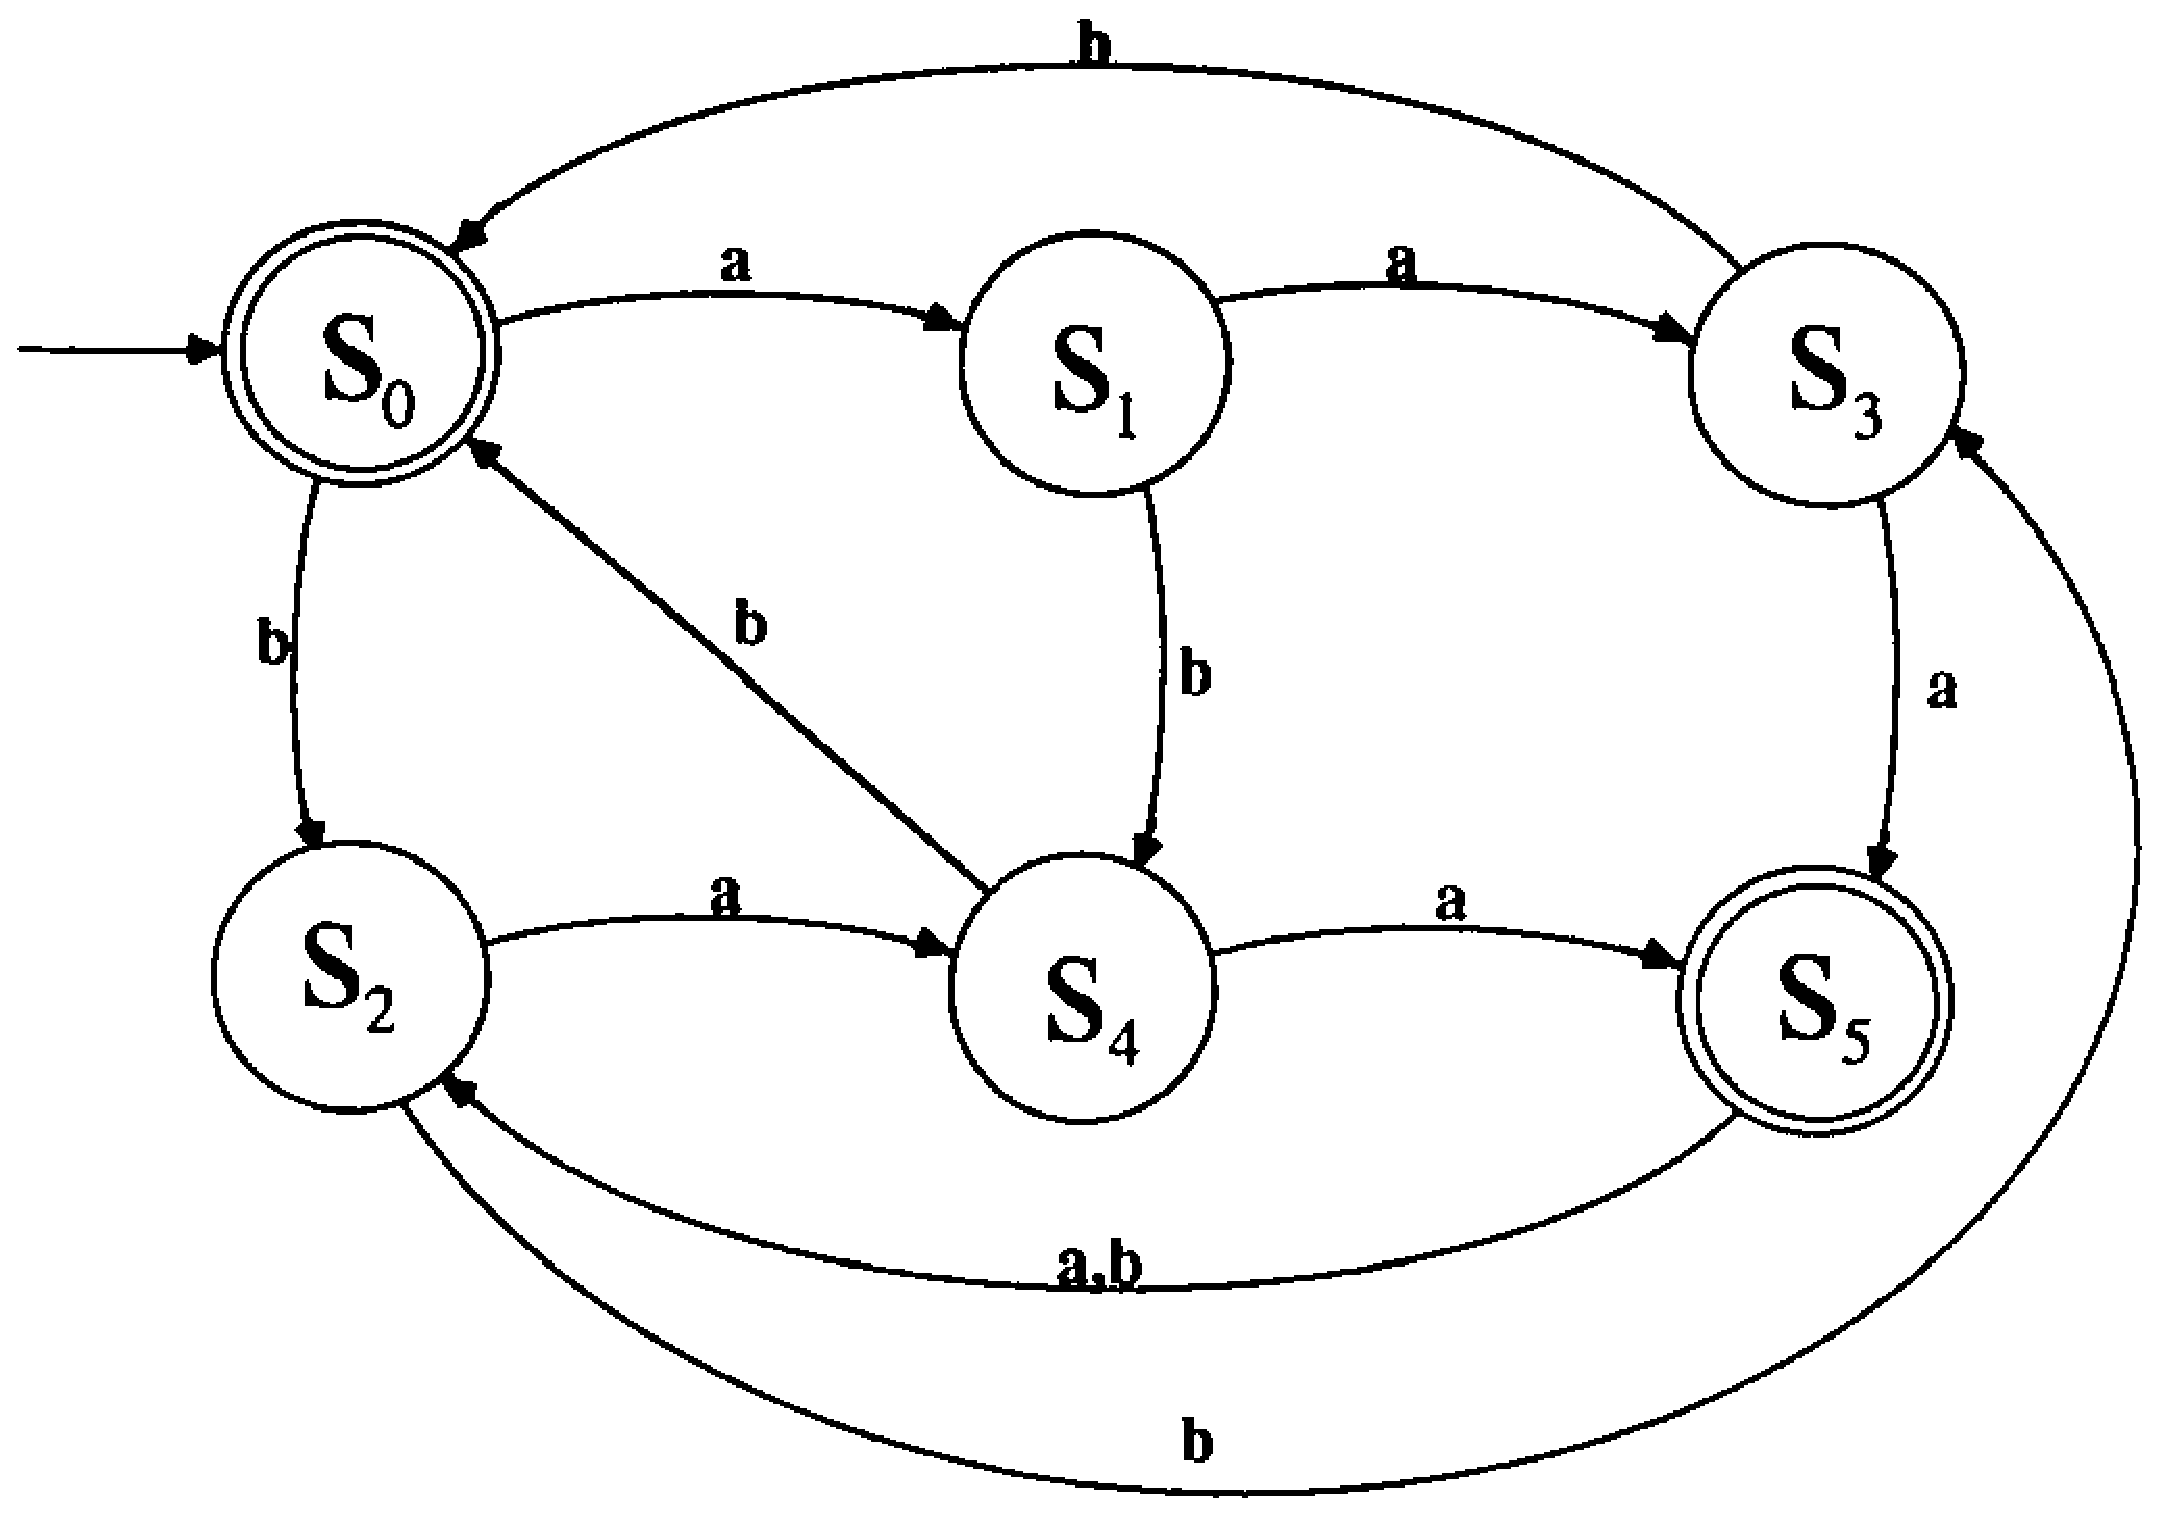
\epsfig{figure=ToFAfigures/fig3-3.eps,width=5in}}
\caption{The second automaton discussed in Example 3.2}\label{fig-3.3}
\end{figure}

% Definition 3.2
\begin{dfn}\label{dfn-3.2}\index{equivalent!DFA states}\index{state equivalence relation!for DFA}
Given a finite automaton $A=\langle\Sigma,S,s_0,\delta,F\rangle$, there is a relation
between the states of $A$ denoted by $E_A$, the \emph{\Index{state equivalence}}
relation on $A$, defined by \\
\centerline{$ (\forall s \in S)(\forall t \in S)(s E_A t \Leftrightarrow
(\forall x \in \Sigma^*)(\DBAR(s,x)\in F \Leftrightarrow \DBAR(t,x)\in F)) $}
\end{dfn}
In other words, we will relate $s$ and $t$ \emph{iff} it is not possible to
distinguish whether we are starting from state $s$ or state $t$; each string
$x \in \Sigma^*$ will \emph{either} take $x$ to a final state when starting from
$s$ and also take $x$ to a final state from $t$, \emph{or} neither $s$ nor $t$ will
take $x$ to a final state.

Another way of looking at this concept is to define new machines that ``look
like'' $A$, but have different start states. Given a finite automaton
$A =\langle\Sigma,S,s_0,\delta,F\rangle$ and two states $s,t \in S$, define a new
automaton $A^t =\langle\Sigma,S,t,\delta,F\rangle$ that has $t$ as a start state, and
another automaton $A^s =\langle\Sigma,S,s,\delta,F\rangle$ having $s$ as a start state.
Then $s E_A t \Leftrightarrow L(A^s) = L(A^t)$. (Why is this an equivalent
definition?) These sets of words will be used in later chapters and are referred
to as \emph{\Index{terminal sets}}. $T(A,t)$ will denote the set of all words
that reach final states from $t$, and thus
$T(A,t) = L(A^t) = \{x\ |\DBAR(t,x) \in F\}$.

In terms of the black box model presented in Chapter \ref{ch-1}, we see that we cannot
distinguish between $A^s$ and $A^t$ by placing matching strings on the input
tapes and observing the acceptance lights of the two machines. For any string,
both $A^s$ and $A^t$ will accept, or both will reject; without looking inside
the black boxes, there is no way to tell whether we are starting in state $s$ or
state $t$. This highlights the sense in which $s$ and $t$ are deemed equivalent:
we cannot distinguish between $s$ and $t$ by the subsequent behavior of the
automaton.

The modified automaton $A^t$, which gives rise to the terminal set $T(A,t)$, can
be contrasted with the modified automaton $A_t=\langle\Sigma,S,s_0,\delta,\{t\}\rangle$
from Chapter \ref{ch-2}, which recognized the initial set
$I(A,t) = \{x\ | \DBAR(s_0,x) = t\}$. Notice that initial sets are comprised of
strings that move from the start state to the distinguished state $t$, while
terminal sets are made up of strings that go from $t$ to a final state.

\subsection*{Example 3.3}

The automaton $N$ discussed in Example 2.6 (Figure \ref{fig-3.4}) has the following
relations comprising $E_N$:
\begin{center}
\begin{tabular}{l}
$s_0 E_N s_0$ \\
$s_1 E_N s_1,$ $s_1 E_N s_2,$ $s_1 E_N s_3$\\
$s_2 E_N s_1,$ $s_2 E_N s_2,$ $s_2 E_N s_3$\\
$s_3 E_N s_1,$ $s_3 E_N s_2,$ $s_3 E_N s_3$
\end{tabular}
\end{center}
This can be succinctly described by listing the equivalence classes:
\begin{center}
\begin{tabular}{l}
$[s_0]_{E_N} = \{s_0\}$ \\
$[s_1]_{E_N} = [s_2]_{E_N} = [s_3]_{E_N} = \{s_1, s_2, s_3\}$,
\end{tabular}
\end{center}
and we will abuse our notation slightly and blur the distinction
between the relation $E_N$ with the partition it generates by writing
$E_N = \{\{s_0\},\{s_1,s_2,s_3\}\}$.

% Figure 3.4
\begin{figure}
\centerline{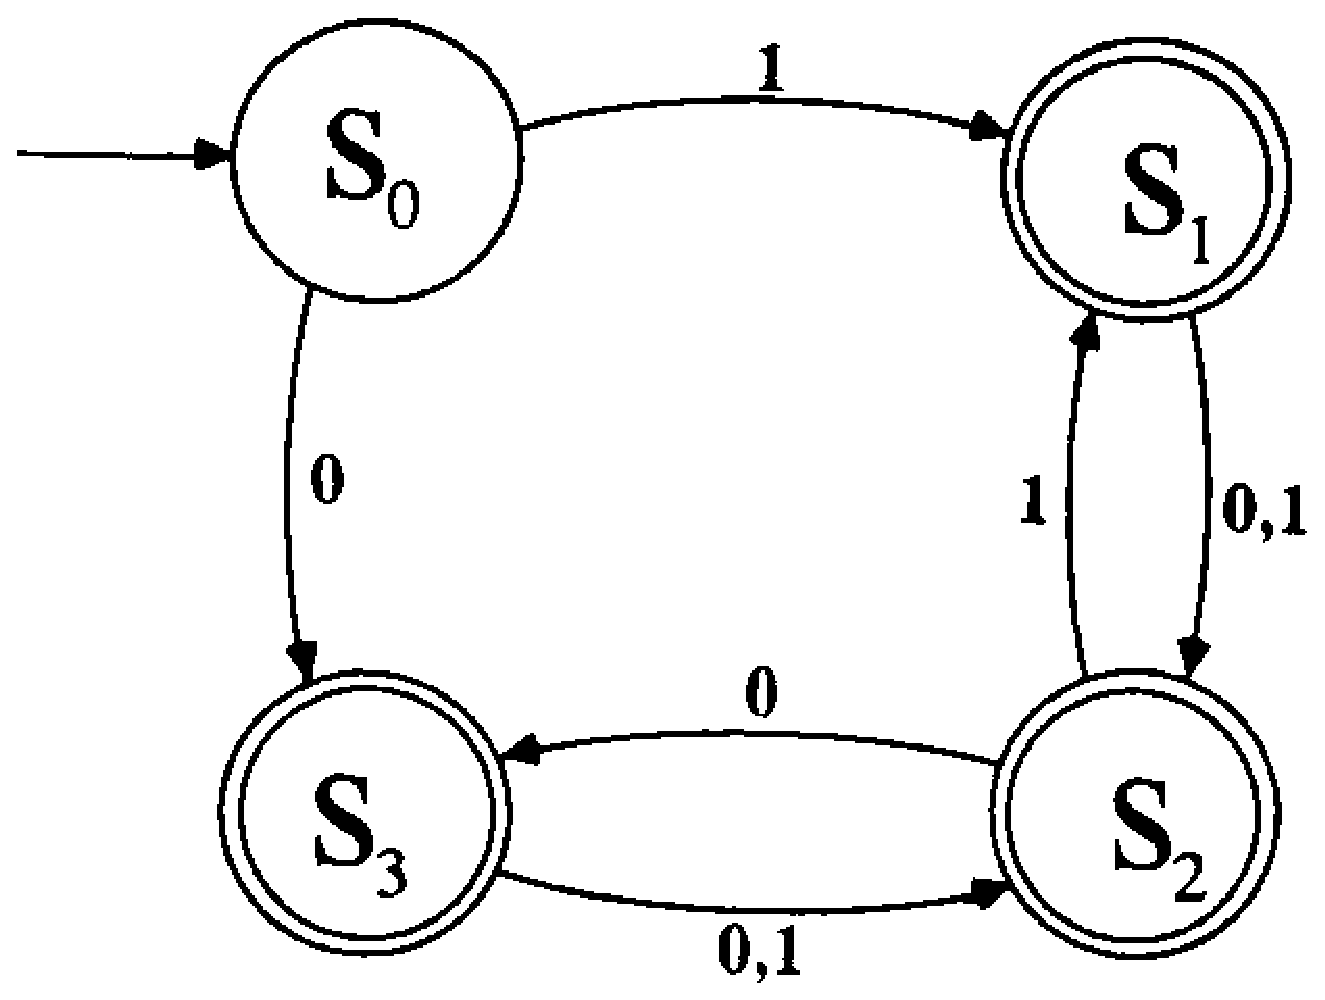
\epsfig{figure=ToFAfigures/fig3-4.eps,width=2.8in}}
\caption{The automaton N discussed in Example 3.3}\label{fig-3.4}
\end{figure}

Recall that Example 2.6 showed that the minimal machine that accepted $L(N)$
had two states; it will be seen that it is no coincidence that $E_N$ has exactly
the same number of equivalence classes.

% Definition 3.3
\begin{dfn}\label{dfn-3.3}\index{reduced!DFA}
A finite automaton $A = \langle\Sigma,S,s_0,\delta,F\rangle$ is called
\emph{reduced} iff $(\forall s,t \in S)(s E_A t \Leftrightarrow s = t)$.
\end{dfn}


In a reduced machine, $E_A$ must be the identity relation on $S$, and in this
case each equivalence class will contain only a single element.

\subsection*{Example 3.4}

The automaton $N$ in Figure \ref{fig-3.4} is not reduced, since Example 3.3 shows that
$[s_2]_{E_N}$ contains three states. On the other hand, the automaton $A$
displayed in Figure \ref{fig-3.5}a is reduced since $[s_0]_{E_A}=\{s_0\}$ and
$[s_1]_{E_A}=\{s_1\}$. The concepts of homomorphism and isomorphism will play an
integral part in justifying the correctness of the algorithms that produce the
optimal DFA for a given language. We need to formalize what we mean when we say
that two automata are ``the same.'' The following examples illustrate the
criteria that must exist between similar machines.

\subsection*{Example 3.5}

We now consider the automaton $B$ shown in Figure \ref{fig-3.5}b, which looks suspiciously
like the DFA $A$ given in Figure \ref{fig-3.5}a. In fact, it is basically the ``same''
machine. While it has been oriented differently (which has no effect on the $\delta$
function), and the start state has been labeled $q_0$ rather than $s_0$, and the
final state is called $q_1$ rather than $s_1$, $A$ and $B$ are otherwise
``identical.'' For such a \emph{\Index{relabeling}} to truly reflect the
same automaton structure, certain conditions must be met, as illustrated in the
following examples.

\subsection*{Example 3.6}

Consider machine $C$, defined by the state transition diagram given in Figure
\ref{fig-3.5}c. This machine is identical to $B$, except for the position of the start
state. However, it is not the same machine as B, since it behaves differently
(and in fact accepts a different language). Thus we see that it is important for
the start state of one machine to correspond to the start state of the other
machine. Note that we cannot circumvent this by letting $q_0$ correspond to
$s_1$, and $q_1$ correspond to $s_0$, since other problems will develop, as
shown next in Example 3.7.

% Figure 3.5
\begin{figure}
\centerline{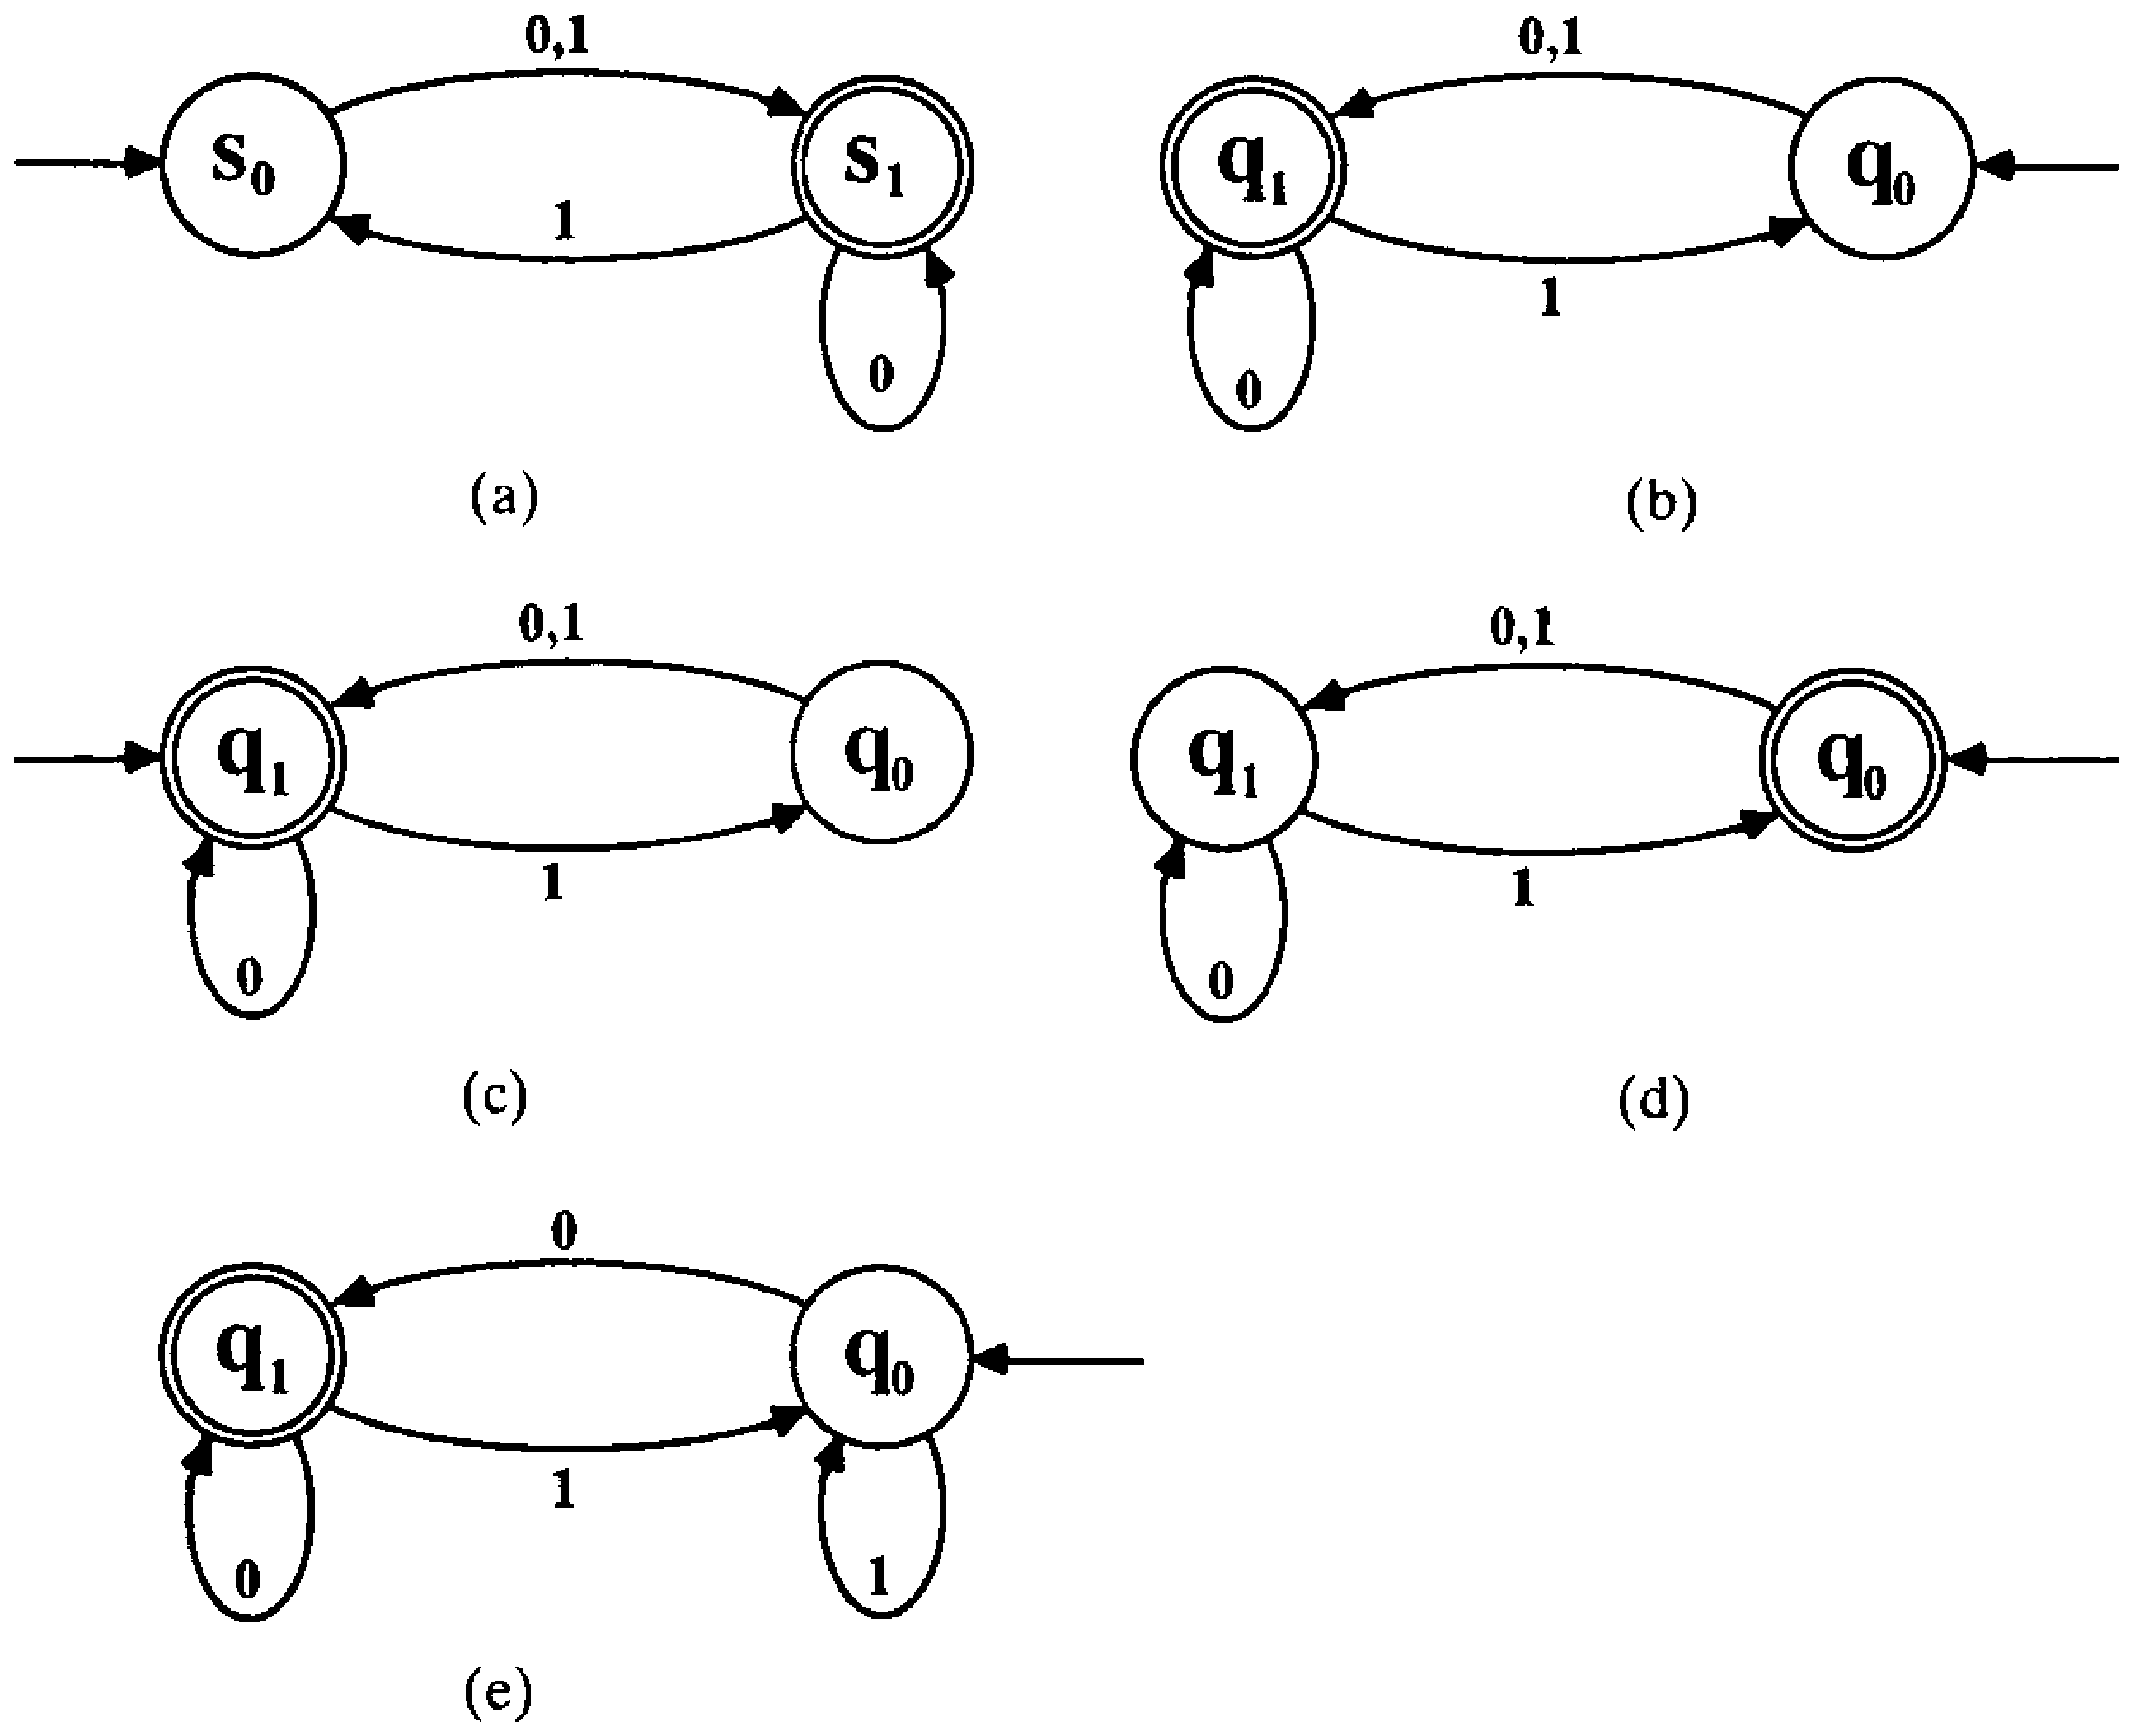
\epsfig{figure=ToFAfigures/fig3-5.eps,width=6in}}
\caption{(a) The automaton A; (b) The automaton B; (c) The automaton C; (d) The
automaton D; (e) The automaton E}\label{fig-3.5}
\end{figure}

\subsection*{Example 3.7}

Let machine $D$ be defined by the state transition diagram given in Figure \ref{fig-3.5}d.
The automata $B$ and $D$ (Figures \ref{fig-3.5}b and \ref{fig-3.5}d) look much the same, with start
states corresponding, but they are not the same (and will in fact accept
different languages), because we cannot get the final states to correspond
correctly. Even if we do get the start and final states to agree, we still have
to make sure that the transitions correspond. This is illustrated in the next
example.

\subsection*{Example 3.8}

Consider the machine $E$ given in Figure \ref{fig-3.5}e. In this automaton, when leaving
the start state, we travel to a final state if we see $\pmb{0}$, and remain at the
start state (which is nonfinal) if we see $\pmb{1}$; this is different from what
happened in machine $A$, where we traveled to a final state regardless of
whether we saw $\pmb{0}$ or $\pmb{1}$. Thus it is seen that we not only have to find
a correspondence (which can be thought of as a function $\mu$) between the
states of our two machines, but we must do this in a way that satisfies the
above three conditions (or else we cannot claim the machines are ``the same'').
This is summed up in the following definition of a \emph{homomorphism}.

% Definition 3.4
\begin{dfn}\label{dfn-3.4}\index{homomorphism!between DFAs}\index{finite automaton!homomorphism}
Given two finite automata, $A=\langle\Sigma,S_A,s_{0_A},\delta_A,F_A\rangle$ and
$B=\langle\Sigma,S_B,s_{0_B},\delta_B,F_B\rangle$, and a function
$\mu:\ S_A \rightarrow S_B$. $\mu$ is called a \emph{finite automata
homomorphism} from $A$ to $B$ iff the following three conditions hold:
\begin{enumerate}[i.]
\item $\mu(s_{0_A}) = s_{0_B}.$
\item $(\forall s \in S_A)(s \in F_A \Leftrightarrow \mu(s) \in F_B).$
\item $(\forall s \in S_A)(\forall \pmb{a} \in \Sigma)(\mu(\delta_A(s,\pmb{a}))
	= \delta_B(\mu(s),\pmb{a})).$
\end{enumerate}
\end{dfn}

Note that $\mu$ is called a homomorphism from $A$ to $B$, but it is actually a
function between state sets, that is, from $S_A$ to $S_B$.

\subsection*{Example 3.9}

Machines $A$ and $B$ in Example 3.5 are homomorphic, since the homomorphism
$\mu$$: \{s_0,s_1\}\rightarrow\{q_0,q_1\}$ defined by $\mu(s_0)=q_0$ and
$\mu(s_1)=q_1$ satisfies the three conditions.

The following example shows that even if we can find a homomorphism that
satisfies the 3 conditions the machines might not be the same.

\subsection*{Example 3.10}

% Figure 3.6
\begin{figure}
\centerline{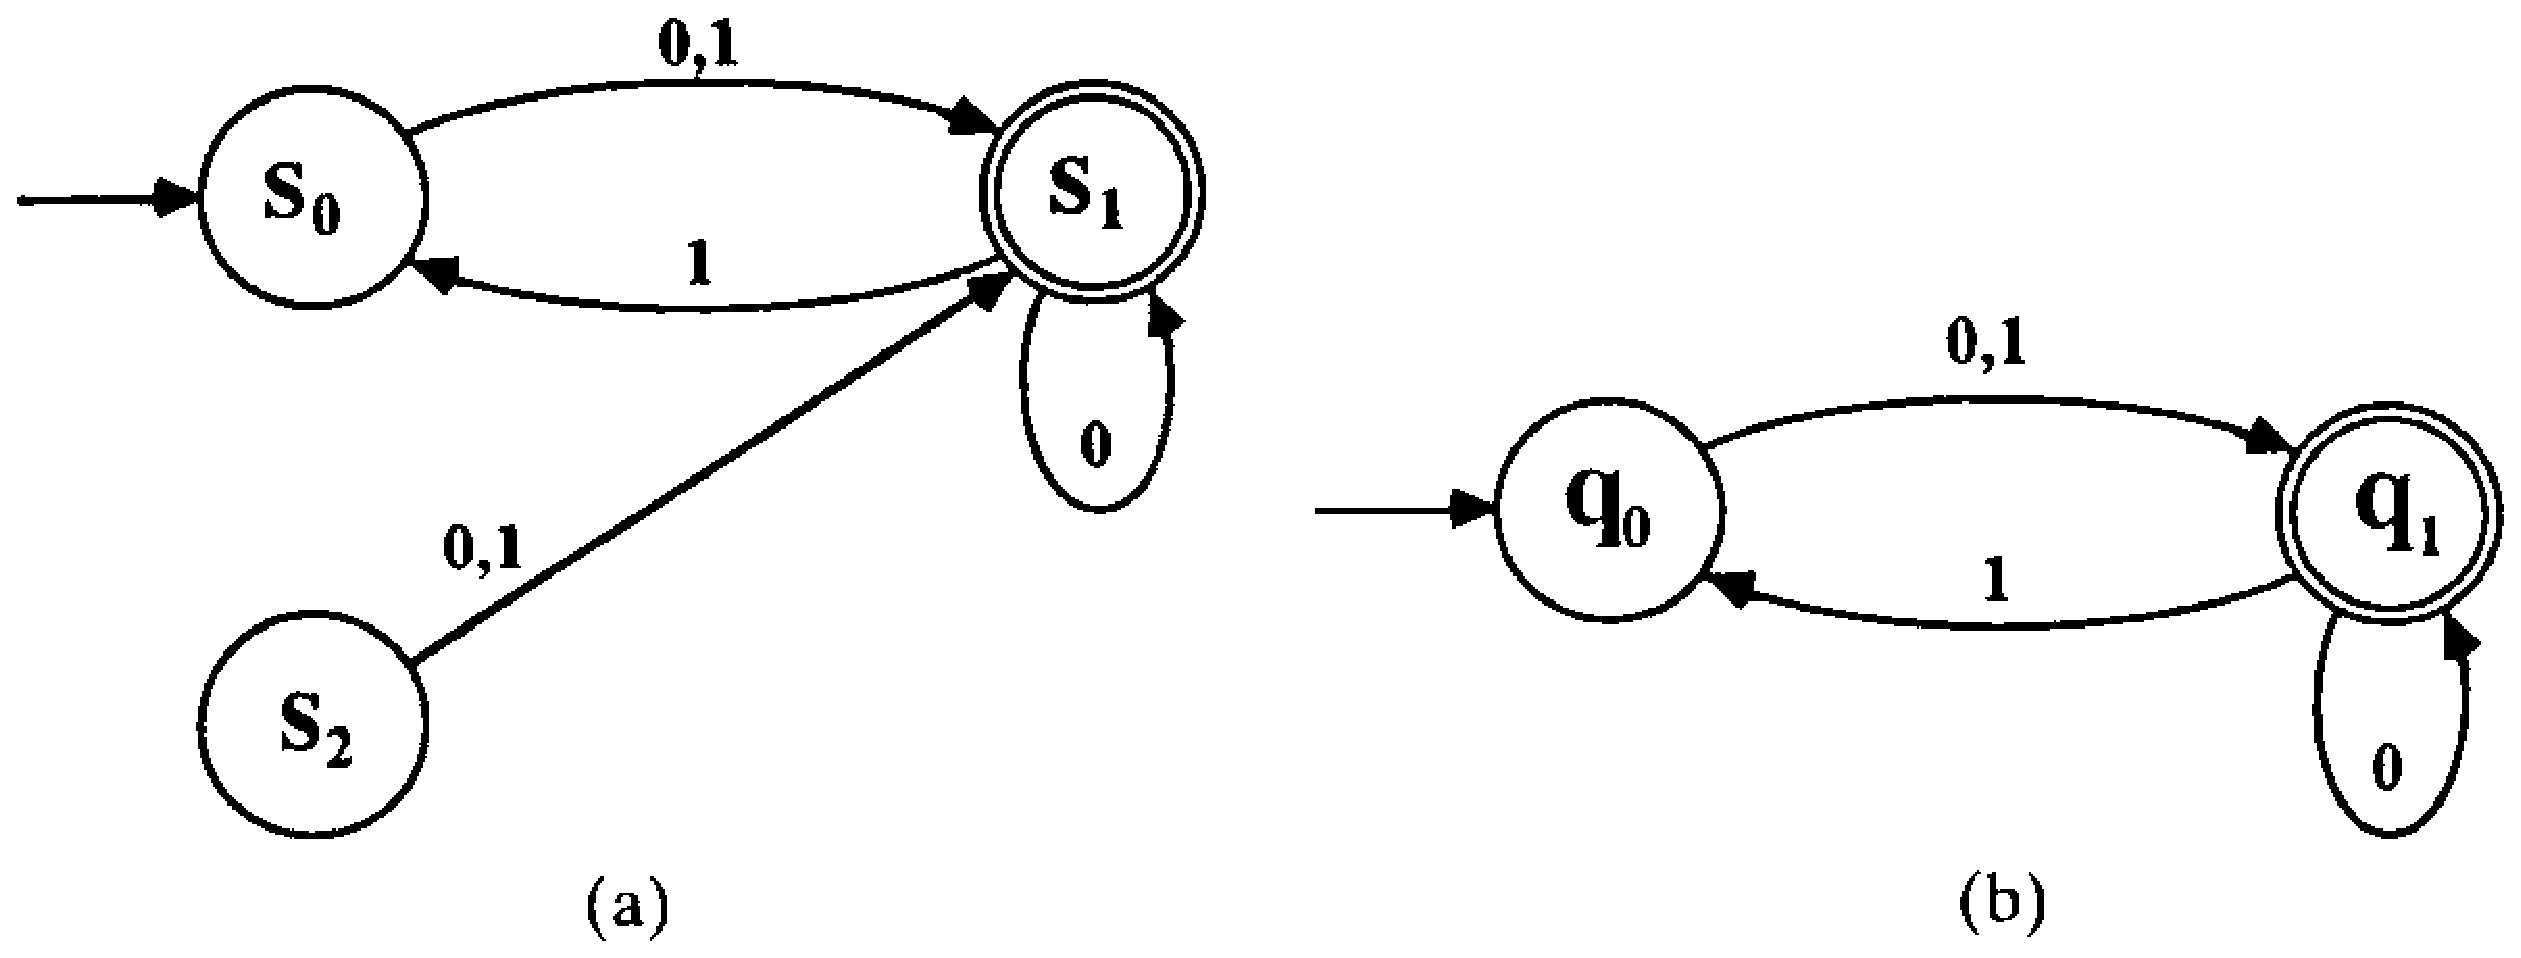
\epsfig{figure=ToFAfigures/fig3-6.eps,width=6in}}
\caption{(a) The DFA $M$ discussed in Example 3.10 (b) The DFA $N$
discussed in Example 3.10}\label{fig-3.6}
\end{figure}

Let $M =\langle\Sigma,\{s_0,s_1,s_2\},s_0,\delta_M,\{s_1\}\rangle$ and
$N =\langle\Sigma,\{q_0,q_1\},q_0,\delta_N,\{q_1\}\rangle$ be given by the state
transition diagrams in Figures \ref{fig-3.6}a and \ref{fig-3.6}b. Define a homomorphism
$\psi$$:\ \{s_0,s_1,s_2\}\rightarrow\{q_0,q_1\}$ by $\psi(s_0)=q_0$,
$\psi(s_1)=q_1$, and $\psi(s_2)=q_0$. Note that the start state maps to the
start state, final states map to final states (and nonfinal states map to
nonfinal states), and, furthermore, the transitions agree. Here is the statement
that the $\pmb{0}$ transition out of state $s_0$ is consistent:
$$ \psi(\delta_M(s_0,\pmb{0}))=\psi(s_1)=q_1=\delta_N(q_0,\pmb{0})=\delta_N(\psi(s_0),\pmb{0}) $$
Note that this really \emph{does} say that the transition labeled $\pmb{0}$
leaving the start state conforms; $s_0$ has a $\pmb{0}$-transition pointing to
$s_1$, and so the $\pmb{0}$-transition from $\psi(s_0)$ should point to $\psi(s_1)$
(that is, $q_0$ should point to $q_1$). But the transition taken from $s_0$
upon seeing a $\pmb{0}$, in our notation, is $\delta_M(s_0,0)$, and the place
$q_0$ goes to is $\delta_N(q_0,0)$. We wish to make sure that the state in $N$
corresponding to where the $\pmb{0}$-transition from $s_0$ points, denoted by
$\psi(\delta_M(s_0,0))$, agrees with the state to which $q_0$ points. Hence we
require $\psi(\delta_M(s_0,0)) = \delta_N(q_0,0)$. In the last formula, $q_0$ was
chosen because that was the state corresponding to $s_0$; that is,
$\psi(s_0)=q_0$. Hence, in our formal notation, we were really checking
$\psi(\delta_M(s_0,0)) = \delta_N(\psi(s_0),0)$. Hence, we see that rule (iii)
requires us to check all transitions leading out of all states for all letters;
that is, $(\forall s \in S_M)(\forall a \in \Sigma)(\psi(\delta_M(s,a)) =
\delta_N(\psi(s),a))$. Applying this rule to each choice of letters $\pmb{a}$ and
states $s$, we have
\begin{center}
\begin{tabular}{l}
$\psi(\delta_M(s_0,\pmb{0}))=\psi(s_1)=q_1=\delta_N(q_0,\pmb{0})=\delta_N(\psi(s_0),\pmb{0})$ \\
$\psi(\delta_M(s_0,\pmb{1}))=\psi(s_1)=q_1=\delta_N(q_0,\pmb{1})=\delta_N(\psi(s_0),\pmb{1})$ \\
$\psi(\delta_M(s_1,\pmb{0}))=\psi(s_1)=q_1=\delta_N(q_1,\pmb{0})=\delta_N(\psi(s_1),\pmb{0})$ \\
$\psi(\delta_M(s_1,\pmb{1}))=\psi(s_0)=q_0=\delta_N(q_1,\pmb{1})=\delta_N(\psi(s_1),\pmb{1})$ \\
$\psi(\delta_M(s_2,\pmb{0}))=\psi(s_1)=q_1=\delta_N(q_0,\pmb{0})=\delta_N(\psi(s_2),\pmb{0})$ \\
$\psi(\delta_M(s_2,\pmb{1}))=\psi(s_1)=q_1=\delta_N(q_0,\pmb{1})=\delta_N(\psi(s_2),\pmb{1})$
\end{tabular}
\end{center}
Hence $\psi$ is a homomorphism between $M$ and $N$ even though $M$ has three
states and $N$ has two states. While the existence of a homomorphism is not
enough to ensure that the machines are ``the same,'' the exercises for this
chapter indicate that the existence of a homomorphism \emph{is} enough to ensure that
the machines are equivalent. The extra condition we need to guarantee that the
machines are identical\index{identical DFAs} (except for a trivial renaming of the states) is that
$\psi$ be a \emph{\Index{bijection}}.

% Definition 3.5
\begin{dfn}\label{dfn-3.5}\index{isomorphism!between DFAs}\index{finite automaton!isomorphism}
Given two finite automata $A=\langle\Sigma,S_A,s_{0_A},\delta_A,F_A\rangle$ and
$B=\langle\Sigma,S_B,s_{0_B},\delta_B,F_B\rangle$, and a function
$\mu:\ S_A \rightarrow S_B$, $\mu$ is called a \emph{finite automata
isomorphism} from $A$ to $B$ iff the following five conditions hold:
\begin{enumerate}[i.]
\item $\mu(s_{0_A}) = s_{0_B}$.
\item $(\forall s \in S_A)(s \in F_A \Leftrightarrow \mu(s) \in F_B)$.
\item $(\forall s \in S_A)(\forall \pmb{a} \in \Sigma)(\mu(\delta_A(s,\pmb{a}))
	= \delta_B(\mu(s),\pmb{a}))$.
\item $\mu$ is a one-to-one function from $S_A$ to $S_B$.
\item $\mu$ is onto $S_B$.
\end{enumerate}
\end{dfn}

\subsection*{Example 3.11}

$\mu$ from Example 3.9 is an isomorphism. Example 3.5 illustrated that the
automaton $A$ was essentially ``the same'' as $B$ except for the way the states
were named. Note that $\mu$ can be thought of as the recipe for relabeling the
states of $A$ to form a machine that would then be in the very strictest sense
absolutely \emph{identical} to $B$. $\psi$ from Example 3.10 is not an
isomorphism because it is not one to one.

% Definition 3.6
\begin{dfn}\label{dfn-3.6}
Given two finite automata $A=\langle\Sigma,S_A,s_{0_A},\delta_A,F_A\rangle$ and
$B=\langle\Sigma,S_B,s_{0_B},\delta_B,F_B\rangle$, $A$ is said to be
\emph{\Index{isomorphic}} to $B$ iff there exists a finite automata isomorphism
between $A$ and $B$, and we will write $A \cong B$.
\end{dfn}

\subsection*{Example 3.12}

Machines $A$ and $B$ from Examples 3.4 and 3.5 are isomorphic. Machines $M$ and
$N$ from Example 3.10 are not isomorphic (and not just because the particular
function $\psi$ fails to satisfy the conditions; we must actually prove that \emph{no}
function exists that qualifies as an isomorphism between $M$ and $N$).

Now that we have rigorously defined the concept of two machines being
``essentially identical,'' we can prove that, given a language $L$, any reduced
and connected machine $A$ accepting $L$ must be \emph{minimal}, that is, have as few
states as possible for that particular language. We will prove this assertion by
showing that any such $A$ is isomorphic to $A_{R_L}$, which was shown in
Corollary \ref{cor-3.2} to be the ``smallest'' possible machine for $L$.


% Theorem 3.1
\begin{thm}\label{thm-3.1}
Let $L$ be any FAD language over an alphabet $\Sigma$, and let
$A=\langle\Sigma,S,s_0,\delta,F\rangle$ be any reduced and connected automaton
that accepts $L$. Then $A \cong A_{R_L}$.

\emph{Proof.} We must try to define a reasonable function $\mu$ from the states
of $A$ to the states of $A_{R_L}$ (which you should recall corresponded to
equivalence classes of $R_L$). A natural way to define $\mu$ (which happens to
work!) is: For each $s \in S$, find a string $x_s \in \Sigma^* \ni
\DBAR(s_0,x_s) = s$. (Since A is connected, we are guaranteed to find such an
$x_s$. In fact, there may be many strings that take us from $s_0$ to $s$; choose
any one of them, and call it $x_s$.) We need to map $s$ to some equivalence
class of $R_L$; the logical choice is the class containing $x_s$. Thus we define
$$ \mu(s)=[x_s]_{R_L} $$
An immediate question comes to mind: There may be several strings that we could
use for $x_s$; does it matter which one we choose to find the equivalence class?
It would not do if, say, $R_L$ consisted of two equivalence classes, the
even-length strings = $[\pmb{11}]_RL$ and the odd-length strings =
$[\pmb{0}]_{R_L}$, and both $\DBAR(s_0,\pmb{0})$ and $\DBAR(s_0,\pmb{11})$ equaled $s$. Then, on
the one hand, $\mu(s)$ should be $[\pmb{0}]_{R_L}$ and, on the other hand, it should
be $[\pmb{11}]_{R_L}$. $\mu$ must be a function; it cannot send $s$ to two different
equivalence classes. Note that there would be no problem if $\DBAR(s_0,\pmb{11})=s$ 
and $\DBAR(s_0,\pmb{1111}) = s$, since $[\pmb{11}]_{R_L}=[\pmb{1111}]_{R_L}$, both of which
represent the set of all even-length strings. Here $x_s$ could be $\pmb{11}$, or
it could be $\pmb{1111}$, and there is no inconsistency in the way in which
$\mu(s)$ is defined; in either case, $s$ is mapped by $\mu$ to the class of
even-length strings. Thus we must first show:
\begin{enumerate}
\item $\mu$ is well-defined (which means it is defined everywhere, and the
definitions are consistent; that is, if there are two choices for $x_s$, say,
$y$ and $z$, then $[y]_{R_L}=[z]_{R_L}$). Since $A$ is connected, each state $s$
can be reached by some string $x_s$; that is,
$(\forall s \in S)(\exists x_s \in \Sigma^*)(\DBAR(s_0,x_s) = s)$, and so there
is indeed (at least) one equivalence class (namely $[x_s]_{R_L}$) to which $s$ maps
under $\mu$. We therefore have $\mu(s)=[x_s]_{R_L}$. Thus $\mu$ is defined
everywhere. We must still make sure that $\mu$ is not multiply defined: Let
$x,y \in \Sigma^*$ and assume $\DBAR(s_0,x)=\DBAR(s_0,y)$. Then
\begin{center}
\begin{tabular}{rcl}
$\DBAR(s_0,x)=\DBAR(s_0,y)$ & $\Rightarrow$ & (by definition of =) \\
$(\forall u \in \Sigma^*)(\DBAR(\DBAR(s_0,x),u) \in F \Leftrightarrow 
\DBAR(\DBAR(s_0,y),u) \in F)$ & $\Rightarrow$ & (by Theorem \ref{thm-1.1}) \\
$(\forall u \in \Sigma^*)(\DBAR(s_0,xu) \in F \Leftrightarrow
\DBAR(s_0,yu) \in F)$ & $\Rightarrow$ & (by definition of $L$) \\
$(\forall u \in \Sigma^*)(xu \in L \Leftrightarrow yu \in L)$ & $\Rightarrow$ &
(by definition of RL) \\
$x\ R_L y$ & $\Rightarrow$ & (by definition of [ ]) \\
$[x]_{R_L} = [y]_{R_L}$ &&
\end{tabular}
\end{center}

Thus, if both $x$ and $y$ take us from $s_0$ to $s$, then it does not matter
whether we let $\mu(s)$ equal $[x]_{R_L}$ or $[y]_{R_L}$, since they are
identical. $\mu$ is therefore a bona fide function.

\item $\mu$ is onto $S_{R_L}$. Every equivalence class must be the image of some
state in $S$, since $(\forall [x]_{R_L}\in S_{R_L})([x]_{R_L}=\mu(\DBAR(s_0,x)))$,
and so $\DBAR(s_0,x)$ maps to $[x]_{R_L}$.

\item $\mu(s_0) = s_{0_{R_L}}$
$$ s_{0_{R_L}} = [\lambda]_{R_L} = \mu(\DBAR(s_0,\lambda)) = \mu(s_0) $$

\item Final states map to final states; that is,
$(\forall s \in S)(\mu(s) \in F_{R_L} \Leftrightarrow s \in F)$. Choose an
$s \in S$ and pick a corresponding $x_s \in \Sigma^*$ such that
$\DBAR(s_0,x_s) = s$. Then
\begin{center}
\begin{tabular}{rcl}
$s \in F$ & $\Leftrightarrow$ & (by definition of $x_s$, and Definition \ref{dfn-1.14}) \\
$x_s \in L(A)$ & $\Leftrightarrow$ & (by definition of L) \\
$x_s \in L$ & $\Leftrightarrow$ & (by definition of $F_{R_L}$) \\
$[x_s]_{R_L} \in F_{R_L}$ & $\Leftrightarrow$ & (by definition of $\mu$) \\
$\mu(s) \in F_{R_L}$ &&
\end{tabular}
\end{center}

\item The transitions match up; that is,
$(\forall s \in S)(\forall a \in \Sigma)(\mu(\delta(s,a)) =
\delta_{R_L}(\mu(s),a))$. Choose an $s \in S$ and pick a corresponding
$x_s \in \Sigma^*$ such that $\DBAR(s_0,x_s) = s$. Note that this implies that
$[x_s]=\mu(s)=\mu(\DBAR(s_0,x_s))$. Then
\begin{center}
\begin{tabular}{rcl}
$\mu(\delta(s,a))$ & $=$ & (by definition of $x_s$) \\
$\mu(\delta(\DBAR(s_0,x_s),a))$ & $=$ & (by Theorem \ref{thm-1.1}) \\
$\mu(\DBAR(s_0,x_s a))$ & $=$ & (by definition of $\mu$) \\
$[x_s a]_{R_L}$ & $=$ & (by definition of $\delta_{R_L}$) \\
$\delta_{R_L}([x_s]_{R_L},a)$ & $=$ & (by definition of $\mu$ and $x_s$) \\
$\delta_{R_L}(\mu(s),a)$ &&
\end{tabular}
\end{center}
So far we have not needed the fact that $A$ was reduced. In fact, we have now
proved that $\mu$ is a homomorphism from $A$ to $A_{R_L}$ as long as $A$ is
merely connected. However, if $A$ is reduced, we can show:

\item $\mu$ is one to one; that is, if $\mu(s)=\mu(t)$, then $s=t$. Let
$s,t \in S$ and assume $\mu(s)=\mu(t)$.
\begin{center}
\begin{tabular}{rcl}
$\mu(s) = \mu(t)$ & $\Rightarrow$ & (by definition of $=$) \\
$(\forall u \in \Sigma^*)(\DBAR_{R_L}(\mu(s),u)=\DBAR_{R_L}(\mu(t),u))$ &
$\Leftrightarrow$ & [by property (5), induction] \\
$(\forall u \in \Sigma^*)(\mu(\DBAR(s,u))=\mu(\DBAR(t,u)))$ & $\Rightarrow$ &
(by definition of $=$) \\
$(\forall u \in \Sigma^*)(\mu(\DBAR(s,u))\in F_{R_L} \Leftrightarrow
\mu(\DBAR(t,u))\in F_{R_L})$ & $\Leftrightarrow$ & [by property (4) above] \\
$(\forall u \in \Sigma^*)(\DBAR(s,u) \in F \Leftrightarrow \DBAR(t,u) \in F)$ &
$\Leftrightarrow$ & (by definition of $E_A$) \\
$s E_A t$ & $\Leftrightarrow$ & (since $A$ is reduced) \\
$s = t$ &&
\end{tabular}
\end{center}
Thus, by results (1) through (6), $\mu$ is a well-defined homomorphism that is
also a bijection; so $\mu$ is an isomorphism and therefore $A \cong A_{R_L}$.
\end{enumerate}
\end{thm}

% Corollary 3.3
\begin{cor}\label{cor-3.3}
Let $A$ and $B$ be reduced and connected finite automata. Under these conditions,
$A$ is equivalent to $B$ iff $A \cong B$.

\emph{Proof}. If $A \cong B$, it is easy to show that $A$ is equivalent to $B$
(as indicated in the exercises, this implication is true even if $A$ and $B$ are
not reduced and connected). Now assume the hypothesis that $A$ and $B$ are
reduced and connected does hold, and that $A$ is equivalent to $B$. Since A is
minimal, $A \cong A_{R_{L(A)}}$. Similarly, $B \cong A_{R_{L(B)}}$. Since
$L(A) = L(B)$, $A_{R_{L(A)}} = A_{R_{L(B)}}$. Therefore,
$A \cong A_{R_{L(A)}} = A_{R_{L(B)}} \cong B$.
\end{cor}

\section{Minimization Algorithms}\label{sec-3.2}

From the results in the previous section, it follows that a reduced and
connected finite automaton must be minimal. This section demonstrates how to
transform an existing DFA into an equivalent machine that is both reduced and
connected and hence is the most efficient machine possible for the given
language. The designer of an automaton can therefore focus solely on producing a
machine that recognizes the correct set of strings (without regard for
efficiency), knowing that the techniques presented in this section can later be
employed to shrink the DFA to its optimal size. The concepts explored in
Chapters \ref{ch-4}, \ref{ch-5}, and \ref{ch-6} will provide further tools to
aid in the design process and corresponding techniques to achieve optimality.

% Corollary 3.4
\begin{cor}\label{cor-3.4}\index{finite automaton!minimal deterministic}
A reduced and connected deterministic finite automaton
$A =\langle\Sigma,S,s_0,\delta,F\rangle$ is minimal.

\emph{Proof.} By Theorem \ref{thm-3.1}, there is an isomorphism between $A$ and $A_{R_L}$.
Since an isomorphism is a bijection between the state sets,
$\|S\| = \|S_{R_L}\|$. By Corollary \ref{cor-3.2}, $A_{R_L}$ has the smallest number of
states, and therefore so does $A$.
\end{cor}

Thus, if we had a machine for $L$ that we could verify was reduced and
connected, we would be able to state that we had found the minimal machine
accepting $L$. We therefore would like some algorithms for determining if a
machine $M$ has these properties. We would also like to find a method for
transforming a nonoptimal machine into one with the desired properties. The
simplest transformation is from a disconnected machine to a connected machine:
given any machine $A$, we will define a connected machine $A^c$ that accepts the
same language that $A$ did; that is, $L(A) =L(A^c)$

% Definition 3.7
\begin{dfn}\label{dfn-3.7}\index{A@$A^c$ (A connected)!for DFA}
Given a finite automaton $A =\langle\Sigma,S,s_0,\delta,F\rangle$, define a new
automaton $A^c =\langle\Sigma,S^c,s^c_0,\delta^c,F^c\rangle$, called A
\emph{connected}, by
\begin{center}
\begin{tabular}{l}
$S^c =\{s\in S$ $|$ $\exists x \in \Sigma^* \ni \DBAR(s_0,x)=s\}$ \\
$s^c_0 = s_0$ \\
$F^c = F \cap S^c =\{f \in F$ $|$ $\exists x \in \Sigma^* \ni \DBAR(s_0,x) = f\}$
\end{tabular}
\end{center}
and $\delta^c$ is derived from the restriction of $\delta$ to $S^c\times\Sigma$:
$$(\forall \pmb{a} \in \Sigma)(\forall s \in S^c)(\delta^c(s, \pmb{a}) = \delta(s,\pmb{a})) $$
\end{dfn}

$A^c$ is thus simply the machine $A$ with the unreachable states ``thrown
away''; $s_0$ can be reached by $x = \lambda$, so it is a valid choice for the
start state in $A^c$. $F^c$ is simply the final states that can be reached from
$s_0$, and $\delta^c$ is the collection of transitions that still come from (and
consequently point to) states in the connected portion. Actually, $\delta^c$ was
defined to be the transitions that merely come from states in $S^c$, with no
mention of any restrictions on the range of $\delta^c$. We must have, however,
$\delta^c: S^c \times \Sigma \rightarrow S^c$; in order for $A^c$ to be well
defined, $\delta^c$ must be shown to map into the proper range. It would not do to
have a transition leading from a state in $A^c$ to a state that is not in the
new state set of $A^c$. The fact that $\delta^c$ does indeed have the desired
properties is relegated to the exercises.

\subsection*{Example 3.13}

Let $M =\langle\{\pmb{a},\pmb{b}\},\{q_0,q_1,q_2,q_3\},q_0,\delta,\{q_1,q_3\}\rangle$, as
illustrated in Figure \ref{fig-3.7}a. By inspection, the only states that can be reached
from the start state are $q_0$ and $q_3$. Hence
$M^c =\langle\{\pmb{a},\pmb{b}\},\{q_0,q_3\},q_0,\delta^c,\{q_3\}\rangle$. The resulting
automaton is shown in Figure \ref{fig-3.7}b. An algorithm for effectively computing $S^c$
will be presented later.

% Figure 3.7
\begin{figure}
\centerline{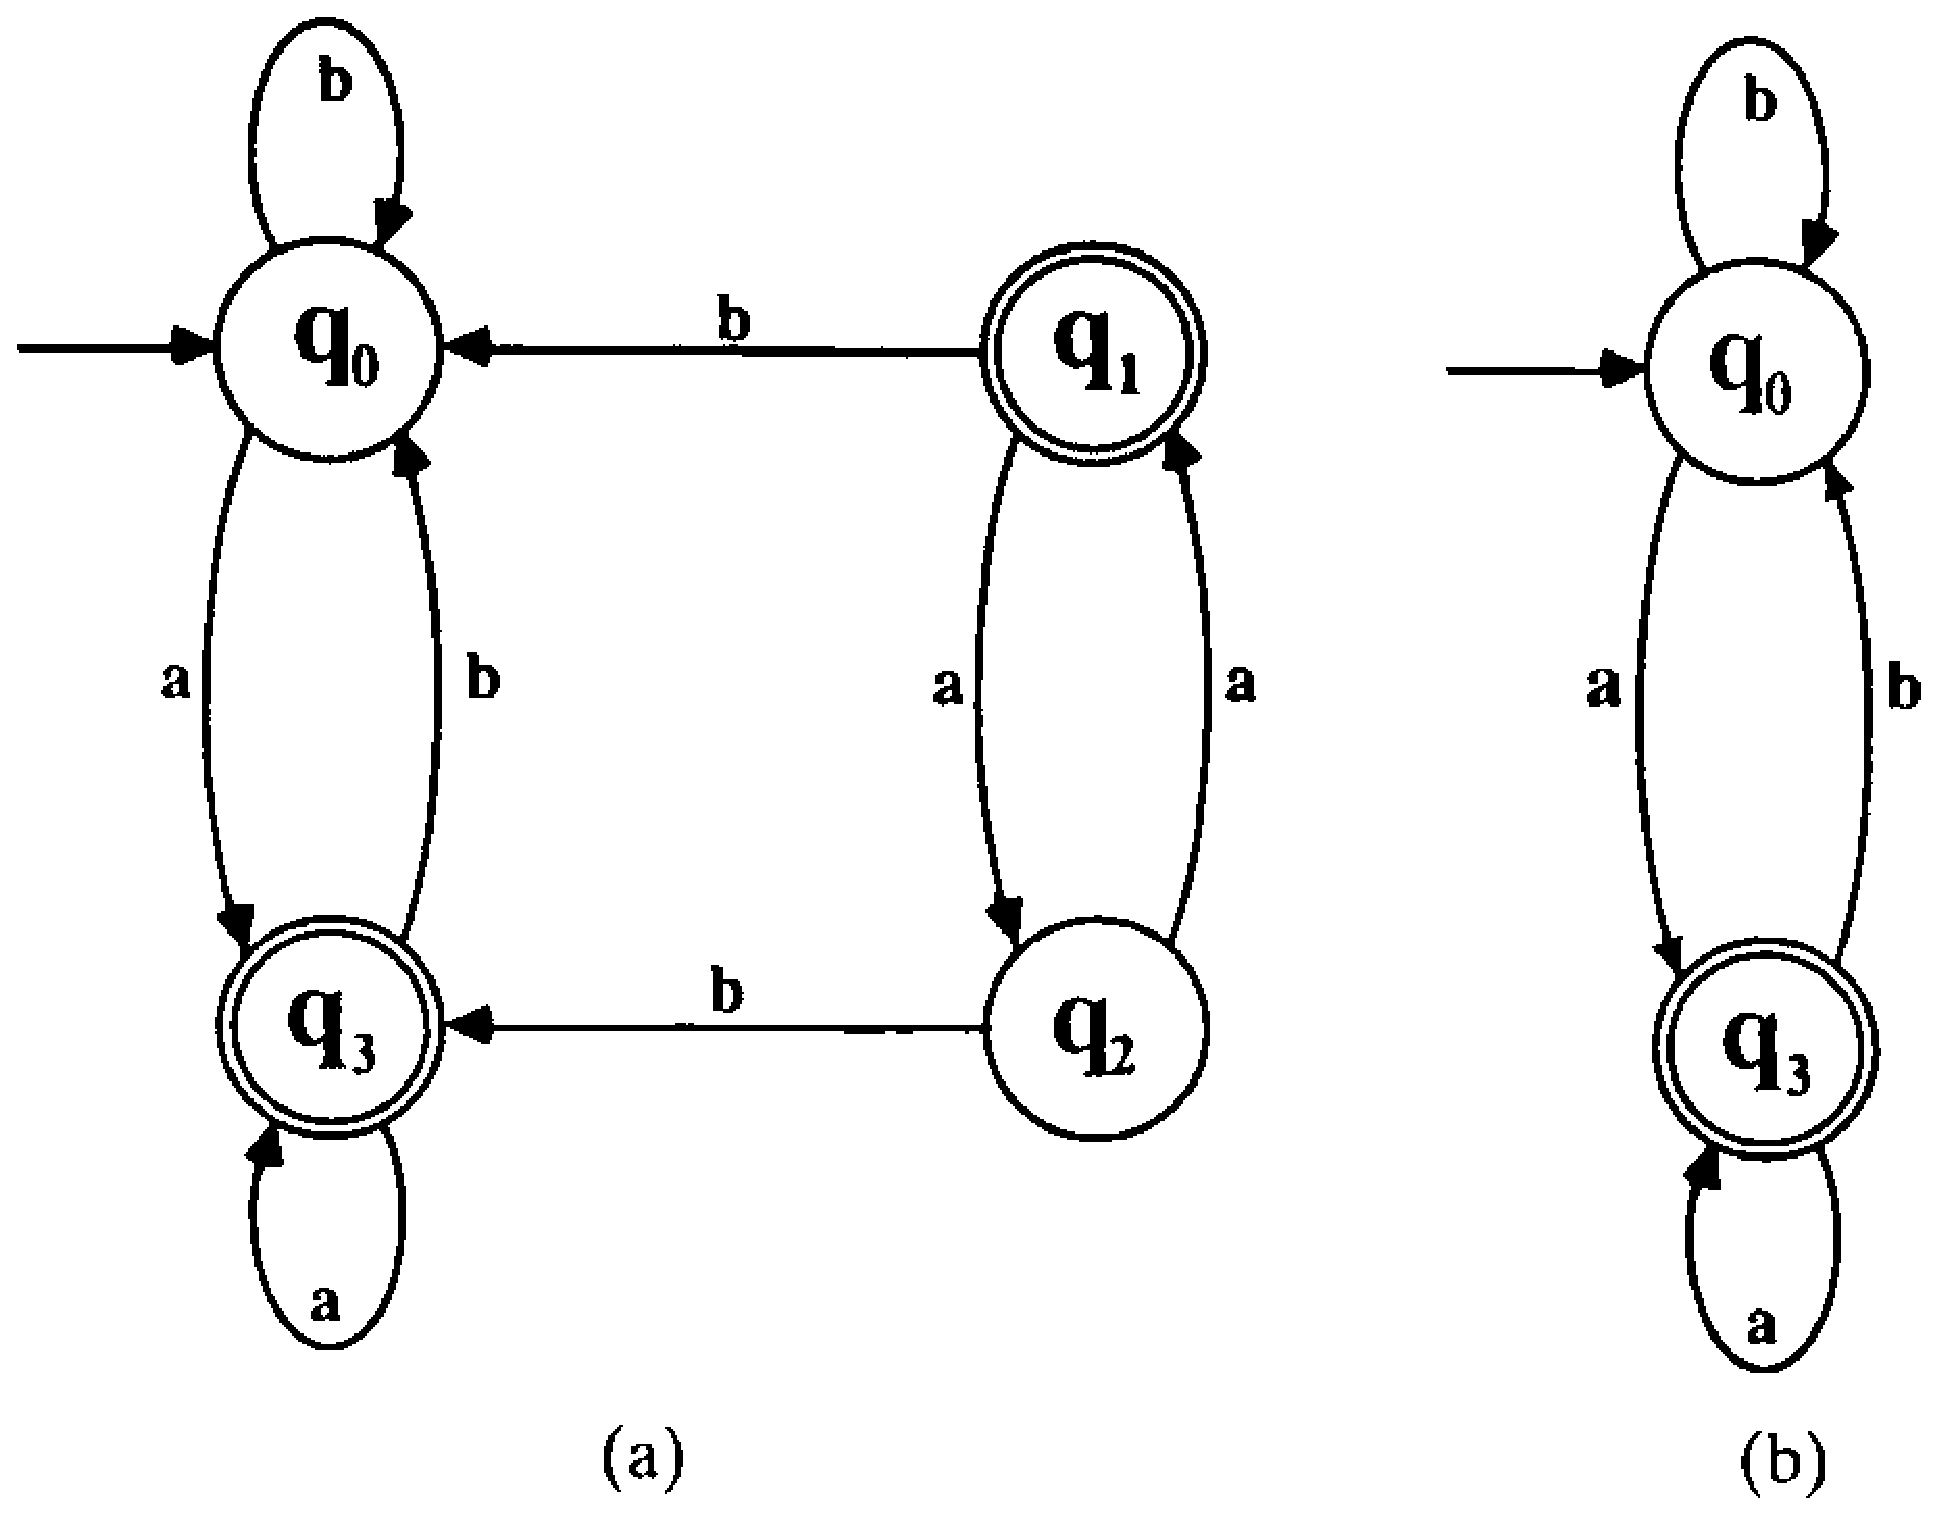
\epsfig{figure=ToFAfigures/fig3-7.eps,width=4in}}
\caption{(a) The DFA $M$ discussed in Example 3.13; (b) The DFA $M^c$ discussed
in Example 3.13}\label{fig-3.7}
\end{figure}

% Theorem 3.2
\begin{thm}\label{thm-3.2}
Given any finite automaton $A$, the new machine $A^c$ is indeed connected.

\emph{Proof.} This is an immediate consequence of the way $S^c$ was defined.
\end{thm}

Definition \ref{dfn-3.7} and Theorem \ref{thm-3.2} would be of little consequence if it were not
for the fact that $A$ and $A^c$ accept the same language. $A^c$ is in fact
equivalent to $A$, as proved in Theorem \ref{thm-3.3}.

% Theorem 3.3
\begin{thm}\label{thm-3.3}\index{equivalent!DFAs}
Given any finite automaton $A =\langle\Sigma,S,s_0,\delta,F\rangle$, $A$ and
$A^c$ are equivalent, that is, $L(A^c) = L(A)$.

\emph{Proof.} Let $x \in \Sigma^*$. Then:
\begin{center}
\begin{tabular}{rcl}
$x \in L(A)$ & $\Leftrightarrow$ & (by definition of $L$) \\
$\exists s \in S \ni (\DBAR(s_0,x) = s \wedge s \in F)$ & $\Leftrightarrow$ &
	(by definition of $S^c$) \\
$s \in S^c \wedge s \in F$ & $\Leftrightarrow$ & (by definition of $\cap$) \\
$s \in (S^c \cap F)$ & $\Leftrightarrow$ & (by definition of $F^c$) \\
$s \in F^c$ & $\Leftrightarrow$ & (by definition of $s$ [above, on line 2]) \\
$\DBAR(s_0,x) \in F^c$ & $\Leftrightarrow$ & (by definition of $\delta^c$ and
	induction) \\
$\DBAR^c(s_0,x) \in F^c$ & $\Leftrightarrow$ & (by definition of $s_0^c$) \\
$\DBAR^c(s_0^c,x) \in F^c$ & $\Leftrightarrow$ & (by definition of $L$) \\
$x \in L(A^c)$ &&
\end{tabular}
\end{center}
\end{thm}

Thus, given any machine $A$, we can find an \emph{equivalent} machine
(that is, a machine that accepts the same language as $A$) that is connected.
Furthermore, there is an algorithm that can be applied to find $A^c$ (that is,
we don't just know that such a machine exists, we actually have a method for
calculating what it is). The definition of $S^c$ implies that there is a
\emph{procedure} for finding $S^c$: one can begin enumerating the strings $x$ in
$\Sigma^*$, and by applying the transition function to each $x$, the new states
that are reached can be included in $S^c$. This is not a very satisfactory
process because there are an infinite number of strings in $\Sigma^*$ to check.
However, the indicated proof for Theorem \ref{thm-2.7} shows that, if a state can be
reached by a ``long'' string, then it can be reached by a ``short'' string.
Thus, we will only need to check the ``short'' strings. In particular,
$$ S^c \equiv \bigcup\limits_{x \in \Sigma^*} \DBAR(s_0,x) =
	\bigcup\limits_{x \in Q} \DBAR(s_0,x) $$
where $Q$ consists of the ``short'' strings:
$Q =\{x \in \Sigma^*|\ |x| < \|S\|\}$. Thus, $Q$ is the set of all strings of
length less than the number of states in the DFA. $Q$ is a finite set, and
therefore we can check all strings $x$ in $Q$ in a finite amount of time; we
therefore have an \emph{algorithm} (that is, a procedure that is guaranteed to halt)
for finding $S^c$, and consequently an algorithm for constructing $A^c$. Thus,
given any machine, we can find an equivalent machine that is connected. The
above method is not very efficient because many calculations are constantly
repeated. A better algorithm based on Definition \ref{dfn-3.10} will be presented later.

We now turn our attention to building a reduced machine from an arbitrary
machine. The following definition gives a consistent way to combine the
redundant states identified by the state equivalence relation $E_A$.

% Definition 3.8
\begin{dfn}\label{dfn-3.8}\index{A @$ A/_{E_A}$ (A modulo $E_A$)!for DFA}
Given a finite automaton $A =\langle\Sigma,S,s_0,\delta,F\rangle$, define a new
finite automaton $A/\!\!_{E_A}$, called \emph{$A$ modulo its state equivalence
relation}, by
$$ A/_{E_A} =\langle\Sigma,S_{E_A},s_{0_{E_A}},\delta_{E_A},F_{E_A}\rangle $$
where
\begin{center}
\begin{tabular}{rcl}
$S_{E_A}$ & $=$ & $\{[s]_{E_A}$ $|$ $s \in S\}$ \\
$s_{0_{E_A}}$ & $=$ & $[s_0]_{E_A}$ \\
$F_{E_A}$ & $=$ & $\{[s]_{E_A}$ $|$ $s \in F\}$
\end{tabular}
\end{center}
and $\delta_{E_A}$ is defined by
$$ (\forall \pmb{a} \in \Sigma)(\forall[s]_{E_A} \in S_{E_A})(\delta_{E_A}([s]_{E_A},\pmb{a}) =
	[\delta(s,\pmb{a})]_{E_A}) $$
\end{dfn}

Thus, there is one state in $A/\!\!_{E_A}$ for each equivalence class in $E_A$, the
new start state is the equivalence class containing $s_0$, and the final states
are those equivalence classes that are made up of states from $F$. The
transition function is also defined in a natural manner: Given an equivalence
class $[t]_{E_A}$ and a letter $\pmb{a}$, choose one state, say $t$, from the class
and see what state the old transition specified $(\delta(t,\pmb{a}))$. The new
transition function will choose the equivalence class containing this new state
$([\delta(t,\pmb{a})]_{E_A})$. Once again, there may be several states in an
equivalence class and thus several states from which to choose. We must make
sure that the definition of $\delta_{E_A}$ does not depend on which state of
$[t]_{E_A}$ we choose (that is, we must ascertain that $\delta_{E_A}$ is well
defined.) Similarly, $F_{E_A}$ should be shown to be well defined (see the
exercises).

It stands to reason that if we coalesce all the states that performed the same
function (that is, were related by $E_A$) into a single state the resulting
machine should no longer have distinct states that perform the same function. We
can indeed prove that this is the case, that is, that $A/_{E_A}$ is reduced.

% Theorem 3.4
\begin{thm}\label{thm-3.4}
Given a finite automaton $A =\langle\Sigma,S,s_0,\delta,F\rangle$, $A/_{E_A}$ is
reduced.

\emph{Proof.} Note that the state equivalence relation for $A/_{E_A}$ is
$E_{(A/\!\!_{E_A}})$, \emph{not} $E_A$. We need to show that if two states of $A/_{E_A}$
are related by the state equivalence relation for $A/\!\!_{E_A}$ then those two
states are identical; that is,
$$ (\forall s,t \in S_{E_A})(s E_{(A/\!_{E_A})} t \Leftrightarrow s = t) $$
Assume $s,t \in S_{E_A}$. Then $\exists s',t' \in S \ni s = [s']_{E_A}$ and
$t = [t']_{E_A}$; furthermore,
\begin{center}
\begin{tabular}{rcl}
$s E_{(A/_{E_A})} t$ & $\Leftrightarrow$ & (by definition of $s',t'$) \\
$[s']_{E_A} E_{(A/_{E_A})} [t']_{E_A}$ & $\Leftrightarrow$ &
	(by definition of $E_{(A/_{E_A})}$) \\
$(\forall x \in \Sigma^*)(\DBAR_{E_A}([s']_{E_A},x) \in F_{E_A} \Leftrightarrow
	\DBAR_{E_A}([t']_{E_A},x) \in F_{E_A})$ & $\Leftrightarrow$ &
	(by $\delta_{E_A}$ and induction) \\
$(\forall x \in \Sigma^*)([\DBAR(s',x)]_{E_A} \in F_{E_A} \Leftrightarrow
	[\DBAR(t',x)]_{E_A} \in F_{E_A})$ & $\Leftrightarrow$ &
	(by definition of $F_{E_A}$) \\
$(\forall x \in \Sigma^*)(\DBAR(s',x) \in F \Leftrightarrow \DBAR(t',x) \in F)$
	& $\Leftrightarrow$ & (by definition of $E_A$) \\
$s' E_A t'$ & $\Leftrightarrow$ & (by definition of $[\ ]$) \\
$[s']_{E_A} = [t']_{E_A}$ & $\Leftrightarrow$ & (by definition of $s,t$) \\
$s = t$ &&
\end{tabular}
\end{center}
\end{thm}

Since we ultimately want to first apply Definition \ref{dfn-3.7} to find a connected DFA
and then apply Definition \ref{dfn-3.8} to reduce that DFA, we wish to show that this
process of obtaining a reduced machine does not destroy connectedness. We can be
assured that if Definition \ref{dfn-3.8} is applied to a connected machine the result will
then be both connected (Theorem \ref{thm-3.5}) and reduced (Theorem \ref{thm-3.4}).

% Theorem 3.5
\begin{thm}\label{thm-3.5}
If $A =\langle\Sigma,S,s_0,\delta,F\rangle$ is connected, then $A/_{E_A}$ is
connected.

\emph{Proof.} We need to show that every state in $A/_{E_A}$ can be reached from
the start state of $A/_{E_A}$. Assume $s \in S_{E_A}$. Then
$\exists s' \in S \ni s = [s']_{E_A}$; but $A$ was connected, and so there
exists an $x \in \Sigma^*$ such that $\DBAR(s_0,x) = s'$; that is, there is a
string that will take us from $s_0$ to $s'$ in the original machine $A$. This
same string will take us from $s_{0_{E_A}}$ to $s$ in $A/_{E_A}$ since
\begin{center}
\begin{tabular}{rcl}
$\DBAR(s_0,x) = s'$ & $\Rightarrow$ & (by definition of $=$) \\
$[\DBAR(s_0,x)]_{E_A} = [s']_{E_A}$ & $\Leftrightarrow$ &
	(by definition of $\delta_{E_A}$ and induction) \\
$\DBAR_{E_A}([s_0]_{E_A},x) = [s']_{E_A}$ & $\Leftrightarrow$ &
	(by definition of $s_{0_{E_A}}$) \\
$\DBAR_{E_A}(s_{0_{E_A}},x) = [s']_{E_A}$ &&
\end{tabular}
\end{center}
Therefore, every state $s \in S_{E_A}$ can be reached from the start state and
$A/_{E_A}$ is thus connected.
\end{thm}

Finally, we want to show that we do not change the language by reducing the
machine. The following theorem proves that $A/_{E_A}$ and $A$ are indeed
equivalent.

% Theorem 3.6
\begin{thm}\label{thm-3.6}\index{equivalent!DFAs}
Given a finite automaton $A =\langle\Sigma,S,s_0,\delta,F\rangle$, then
$L(A/_{E_A}) = L(A)$.

\emph{Proof.}
\begin{center}
\begin{tabular}{rcl}
$x \in L(A/_{E_A})$ & $\Leftrightarrow$ & (by definition of $L$) \\
$\DBAR_{E_A}(s_{0_{E_A}},x) \in F_{E_A}$ & $\Leftrightarrow$ &
	(by definition of $s_{0_{E_A}}$) \\
$\DBAR_{E_A}([s_0]_{E_A},x) \in F_{E_A}$ & $\Leftrightarrow$ &
	(by definition of $\delta_{E_A}$ and induction) \\
$[\DBAR(s_0,x)]_{E_A} \in F_{E_A}$ & $\Leftrightarrow$ &
	(by definition of $F_{E_A}$) \\
$\DBAR(s_0,x) \in F$ & $\Leftrightarrow$ & (by definition of $L$) \\
$x \in L(A)$ &&
\end{tabular}
\end{center}
\end{thm}

% Theorem 3.7
\begin{thm}\label{thm-3.7}\index{finite automaton!minimal deterministic}
Given a finite automaton definable language $L$ and any finite automaton $A$
that accepts $L$, then there exists an algorithm for constructing the \emph{unique}
(up to isomorphism) minimum-state finite automaton accepting $L$.

\emph{Proof.} For the finite automaton $A$ that accepts $L$, there is an
algorithm for finding the set of connected states in $A$, and therefore there
exists an algorithm for constructing $A^c$, which is a \emph{connected} automaton with
the property that $L(A^c) = L(A) = L$.

Furthermore, there exists an algorithm for computing $E_{A^c}$ the state equivalence
relation on $A^c$; consequently, there is an algorithm for constructing
$A^c\!/\!_{E_{A^c}}$, which is a reduced, connected automaton with the property that
$L(A^c\!/\!_{E_{A^c}}) \cong L(A^c) = L(A) = L$

From the main theorem on minimization (Theorem \ref{thm-3.1}), we know that
$A^c\!/\!_{E_{A^c}} \cong A_{R_L}$, and $A_{R_L}$ is the unique (up to isomorphism)
minimum-state finite automaton accepting $L$. Consequently, the derived
automaton $A^c/\!_{E_{A^c}}$ is likewise a minimum-state automaton.
\end{thm}

The remainder of the chapter is devoted to developing the methods for computing
$S^c$ and $E_A$ and justifying that the resulting algorithms are indeed correct.

Our formal definition of $E_A$ requires that an infinite number of strings be
checked before we can find the equivalence classes upon which $A^c\!/\!_{E_{A^c}}$
is based. If we could find an algorithm to generate $E_A$, we would then have an
algorithm for building the minimal machine. This is the motivation for
Definition \ref{dfn-3.9}.

% Definition 3.9
%\begin{dfn}\label{dfn-3.9}\index{i\raisebox{0.6ex}{\em\scriptsize th} partial state equivalence relation (DFA)}
\begin{dfn}\label{dfn-3.9}\index{i\textsuperscript{th} partial state equivalence relation (DFA)}
Given a finite automaton $A =\langle\Sigma,S,s_0,\delta,F\rangle$ and an integer
$i$, define the \emph{i\textsuperscript{th} partial state equivalence relation on A}, a
relation between the states of $A$ denoted by $E_{iA}$, by
$$ (\forall s,t \in S)(sE_{iA}t \ \ \ \emph{iff}\ \ \  (\forall x \in \Sigma^* \ni |x|
	\leq  i)(\DBAR(s,x) \in F \Leftrightarrow \DBAR(t,x) \in F)) $$
\end{dfn}

Thus $E_{iA}$ relates states that cannot be distinguished by strings of length
$i$ or less. Contrast this to the definition of $E_A$, which related states that
could not be distinguished by any string of any length. $E_{0A}$ denotes a
relatively weak criterion that is progressively strengthened with successive
$E_{iA}$ relations. As illustrated by Example 3.14, these relations culminate in
the relation we seek, $E_A$.

\subsection*{Example 3.14}

Let $B$ be the DFA illustrated in Figure \ref{fig-3.8}. Consider the relation $E_{0B}$.
The empty string $\lambda$ can differentiate between $q_0$ and the final states,
but cannot differentiate between $q_1,\ q_2,\ q_3$, and $q_4$. Thus $E_{0B}$ has
two equivalence classes, $\{q_0\}$ and $\{q_1, q_2, q_3, q_4\}$.

In $E_{1B}$, $\lambda$ still differentiates $q_0$ from the other states, but the
string \pmb{1} can distinguish $q_3$ from $q_1,\ q_2$, and $q_4$ since
$\DBAR(q_3,\pmb{1}) \notin F$, but $\DBAR(q_i,\pmb{1}) \in F$ for $i$ = 1, 2, and 4. We
still cannot distinguish between $q_1,\ q_2$, and $q_4$ with strings of length
0 or 1, so these remain together and
$E_{1B}=\{\{q_0\},\{q_3\},\{q_1,q_2,q_4\}\}$. Similarly, since
$\DBAR(q_1,\pmb{11})\in F$ but $\DBAR(q_2,\pmb{11})\notin F$ and $\DBAR(q_4,\pmb{11})\notin F$,
$E_{2B}=\{\{q_0\},\{q_3\},\{q_1\},\{q_2,q_4\}\}$. Further investigation shows
$E_{2B} = E_{3B} = E_{4B} = E_{5B} = \cdots$, and indeed $E_B = E_{2B}$.

% Figure 3.8
\begin{figure}
\centerline{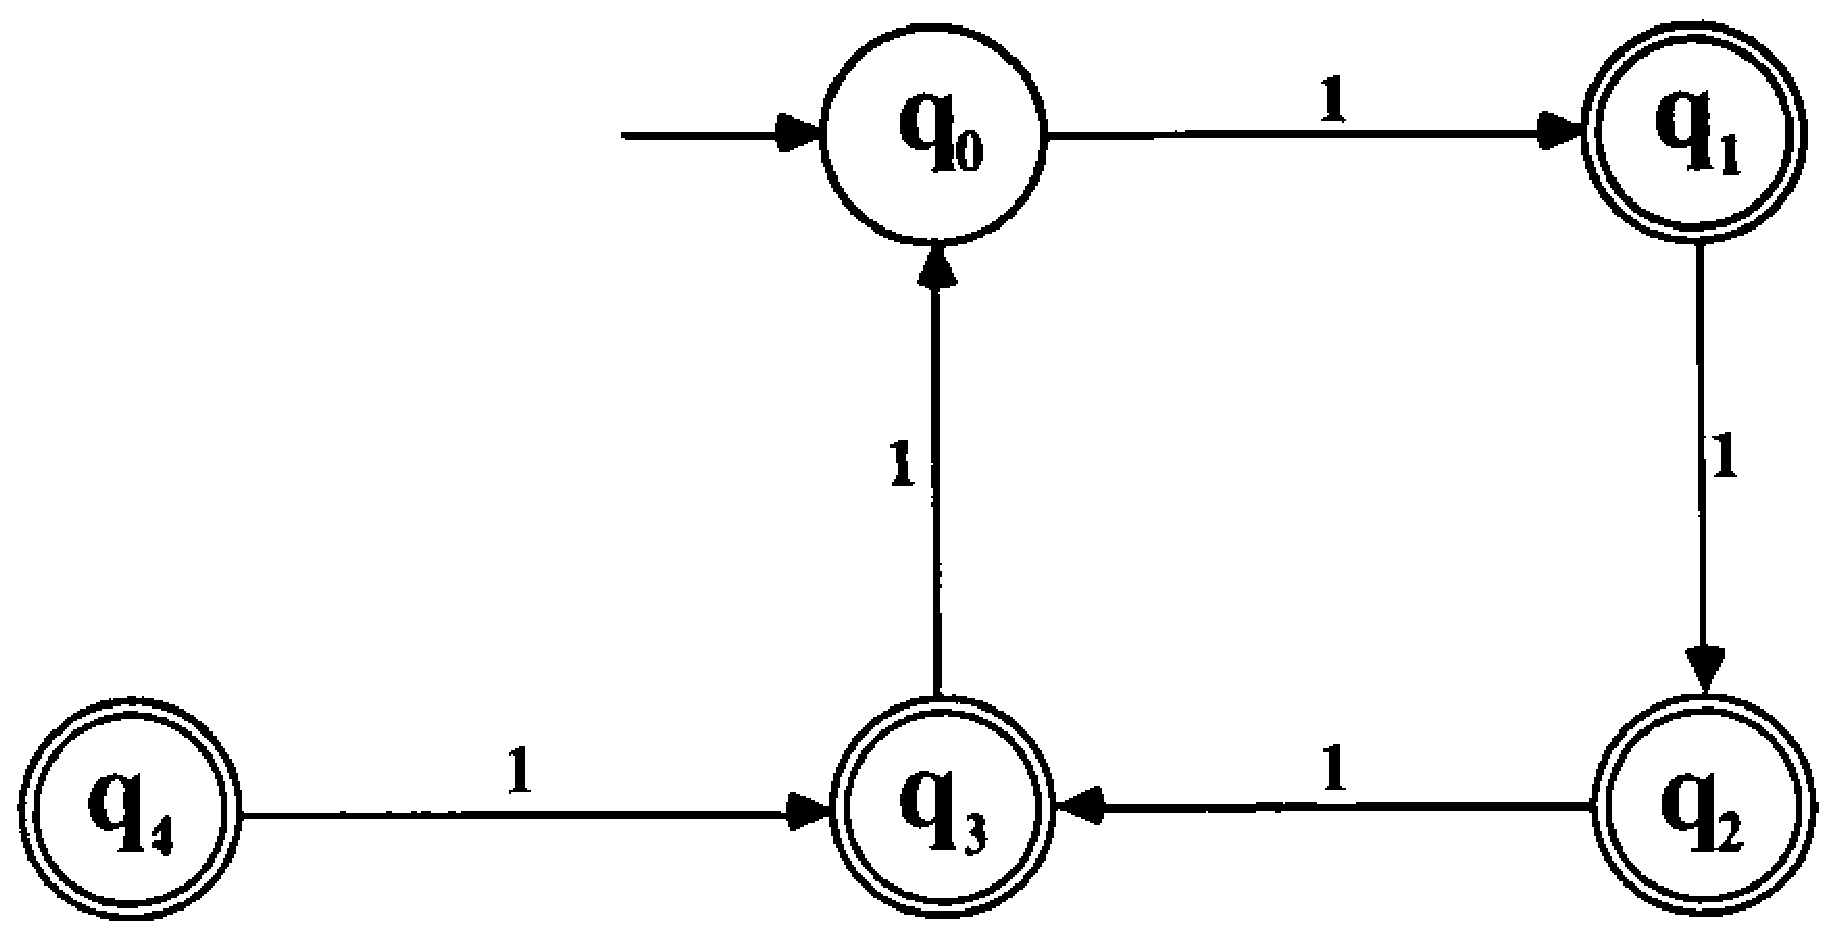
\epsfig{figure=ToFAfigures/fig3-8.eps,width=4in}}
\caption{The DFA B discussed in Example 3.14}\label{fig-3.8}
\end{figure}

The $i$th state equivalence relation provides a convenient vehicle for computing
$E_A$. The behavior exhibited by the relations in Example 3.14 follow a pattern
that is similar for all deterministic finite automata. The following
observations will culminate in a proof that the calculation of successive
partial state equivalence relations is guaranteed to lead to the relation $E_A$.

Given an integer $i$ and a finite alphabet $\Sigma$, there is clearly an
\emph{algorithm} for finding $E_{iA}$ since there are only a finite number of
strings in $\Sigma^0 \cup \Sigma^1 \cup \Sigma^2 \cup \cdots \cup \Sigma^i$.
Furthermore, given every $E_{iA}$, there is an expression for $E_A$:
$$ E_A = E_{0A} \cap E_{1A} \cap E_{2A} \cap E_{3A} \cap \cdots \cap E_{nA} \cap
	\cdots = \bigcap\limits^\infty_{j=0} E_{jA} $$
The proof is relegated to the exercises and is related to the fact that
$$ \Sigma^*=\Sigma^0\cup\Sigma^1\cup\Sigma^2\cup\cdots\cup\Sigma^n\cup\cdots $$
Finally, it should be clear that if two states cannot be distinguished by
strings of length 7 or less, they cannot be distinguished by strings of length 6
or less, which means $E_{7A}$ is a refinement of $E_{6A}$. This principle
generalizes, as formalized below.

% Lemma 3.1
\begin{lmm}\label{lmm-3.1}
Given a finite automaton $A =\langle\Sigma,S,s_0,\delta,F\rangle$ and an integer
$m$, $E_{m+1A}$ is a refinement of $E_{mA}$, which means
$$ (\forall s,t \in S)(s E_{m+1A}t \Rightarrow s E_{mA}t) $$
or
$$ E_{m+1A} \subseteq E_{mA} $$
\emph{Proof.} See the exercises.
\end{lmm}

Lemma \ref{lmm-3.2} shows that each $E_{mA}$ is related to the desired $E_A$. Lemma \ref{lmm-3.1}
thus shows that successive $E_{mA}$ relations come closer to ``looking like''
$E_A$.

% Lemma 3.2
\begin{lmm}\label{lmm-3.2}
Given a finite automaton $A =\langle\Sigma,S,s_0,\delta,F\rangle$ and an integer
$m$, $E_A$ is a refinement of $E_{mA}$, and so
$$ (\forall s,t \in S)(s E_A t \Rightarrow s E_{mA} t) $$
That is,
$$ E_A \subseteq E_{mA} $$

\emph{Proof.} Let $s,t \in S$. Then
\begin{center}
\begin{tabular}{rcl}
$s E_A t$ & $\Rightarrow$ & (by definition of $E_A$) \\
$(\forall x \in \Sigma^*)(\DBAR(s,x) \in F \Leftrightarrow \DBAR(t,x) \in F)$ &
  $\Rightarrow$ & (true for all $x$, so it is true for all ``short'' $x$)\\
$(\forall x \in \Sigma^* \ni |x| \leq m)(\DBAR(s,x) \in F \Leftrightarrow
\DBAR(t,x) \in F)$ & $\Rightarrow$ & (by definition of $E_{mA}$) \\
$s E_{mA} t$
\end{tabular}
\end{center}
\end{lmm}

While it is clearly possible to find a given $E_{mA}$ by applying the definition
to each of the strings in $\Sigma^0 \cup \Sigma^1 \cup \Sigma^2 \cup \cdots
\Sigma^m$, there is a much more efficient way if $E_{m-1A}$ is already known, as
outlined in Theorem \ref{thm-3.8}. A starting point is provided by $E_{0A}$, which can be
found very easily, as shown by Lemma \ref{lmm-3.3}. From $E_{0A}$, $E_{1A}$ can then be
found using Theorem \ref{thm-3.8}, and then $E_{2A}$, and so on.

% Lemma 3.3
\begin{lmm}\label{lmm-3.3}
Given a finite automaton $A=\langle\Sigma,S,s_0,\delta,F\rangle$, $E_{0A}$ has
two equivalence classes, $F$ and $S-F$ (unless either $F$ or $S-F$ is empty, in
which case there is only one equivalence class, $S$).

\emph{Proof.} The proof follows immediately from the definition of $E_{0A}$; the
empty string $\lambda$ differentiates between final and nonfinal states,
producing the equivalence classes outlined above.
\end{lmm}

Given $E_{0A}$ as a starting point, Theorem \ref{thm-3.8} shows how successive relations
can be efficiently calculated.

% Theorem 3.8
\begin{thm}\label{thm-3.8}
Given a finite automaton $A =\langle\Sigma,S,s_0,\delta,F\rangle$,
$$(\forall s\in S)(\forall t\in S)(\forall i \in\NN)(s E_{i+1A} t\Leftrightarrow
s E_{iA} t \wedge (\forall \pmb{a} \in \Sigma)(\delta(s,\pmb{a})E_{iA}\delta(t,\pmb{a}))) $$

\emph{Proof.} Let $s \in S,\ t \in S$. Then
\begin{center}
\begin{tabular}{rcl}
$s E_{i+1A} t$ & $\Leftrightarrow$ & $(\forall x \in \Sigma^* \ni |x| \leq i+1)
(\DBAR(s,x) \in F \Leftrightarrow \DBAR(t,x) \in F)$ \\
& $\Leftrightarrow$ & $(\forall x \in \Sigma^* \ni |x| \leq i)[\DBAR(s,x) \in F
\Leftrightarrow \DBAR(t,x) \in F] \wedge$ \\
&& $(\forall y \in \Sigma^* \ni |y| = i+1)[\DBAR(s,y) \in F \Leftrightarrow
\DBAR(t,y) \in F]$ \\
& $\Leftrightarrow$ & $(\forall x \in \Sigma^* \ni |x| \leq i)[\DBAR(s,x) \in F
\Leftrightarrow \DBAR(t,x) \in F] \wedge$ \\
&& $(\forall y \in \Sigma^* \ni 1 \leq |y| \leq i+1)[\DBAR(s,y)\in F
\Leftrightarrow \DBAR(t,y)\in F]$ \\
& $\Leftrightarrow$ & $(\forall x \in \Sigma^* \ni |x| \leq i)[\DBAR(s,x) \in F
\Leftrightarrow \DBAR(t,x) \in F] \wedge$ \\
&& $(\forall \pmb{a} \in \Sigma)(\forall x \in \Sigma^* \ni |x| \leq i)[\DBAR(s,\pmb{a}x)
\in F \Leftrightarrow \DBAR(t,\pmb{a}x) \in F]$ \\
& $\Leftrightarrow$ & $s E_{iA} t \wedge$ \\
&& $(\forall \pmb{a} \in \Sigma)(\forall x \in \Sigma^* \ni |x| \leq i)(\DBAR(s,\pmb{a}x)
\in F \Leftrightarrow \DBAR(t,\pmb{a}x) \in F)$ \\
& $\Leftrightarrow$ & $s E_{iA} t \wedge$ \\
&& $(\forall \pmb{a} \in \Sigma)(\forall x \in \Sigma^* \ni |x| \leq i)
(\DBAR(\delta(s,\pmb{a}),x) \in F \Leftrightarrow \DBAR(\delta(t,\pmb{a})x) \in F)$ \\
& $\Leftrightarrow$ & $s E_{iA} t \wedge (\forall \pmb{a} \in \Sigma)(\delta(s,\pmb{a})
E_{iA} \delta(t,\pmb{a}))$
\end{tabular}
\end{center}
\end{thm}

Note that Theorem \ref{thm-3.8} gives a far superior method for determining successive
$E_{iA}$ relations. The definition required the examination of many (long)
\emph{strings} using the $\DBAR$ function; Theorem \ref{thm-3.8} allows us to simply check
a few \emph{letters} using the $\delta$ function, without needing $\DBAR$ at all. Theorems \ref{thm-3.9},
\ref{thm-3.10}, and \ref{thm-3.11} will assure us that $E_A$ will eventually be
found. The following theorem guarantees that the relations, should they ever
begin to look alike, will continue to look alike as successive relations are
computed.

% Theorem 3.9
\begin{thm}\label{thm-3.9}
Given a finite automaton $A =\langle\Sigma,S,s_0,\delta,F\rangle$,
$$ (\exists m \in \NN \ni E_{mA} = E_{m+1A}) \Rightarrow
	(\forall k \in \NN)(E_{m+kA} = E_{mA}) $$

\emph{Proof.} By induction on $k$; see the exercises.
\end{thm}

The result in Theorem \ref{thm-3.9} is essential to the proof of the next
theorem, which guarantees that when successive relations look alike they are
identical to $E_A$.

% Theorem 3.10
\begin{thm}\label{thm-3.10}
Given a finite automaton $A =\langle\Sigma,S,s_0,\delta,F\rangle$,
$$ (\exists m \in \NN \ni E_{mA}=E_{m+1A}) \Rightarrow E_{mA}=E_A $$

\emph{Proof.} Assume $\exists m \in \NN \ni E_{mA}=E_{m+1A}$ and let
$q,r \in S$:
\begin{enumerate}
\item By Lemma \ref{lmm-3.2}, $q E_A r \Rightarrow q E_{mA} r$.
\item Conversely, assume $q E_{mA} r$. Then
\begin{center}
\begin{tabular}{rl}
$q E_{mA}r$ & $\Rightarrow$ (by assumption) \\
$q E_{m+lA} r$ & $\Rightarrow$ (by Theorem \ref{thm-3.9}) \\
$(\forall j \geq m)(q E_{jA} r)$ &
\end{tabular}
\end{center}
Furthermore, by Lemma \ref{lmm-3.1}, $(\forall j \leq m)(q E_{jA} r)$, and so
$(\forall j \in \NN)(q E_{jA} r)$; but by definition or $E_A$, this implies
$q E_A r$. We have just shown that $q E_{mA} r \Rightarrow q E_A r$.
\item Combining (1) and (2), we have
$(\forall q,r \in S)(q E_{mA} r \Leftrightarrow q E_A r)$, and so $E_{mA}=E_A$.
\end{enumerate}
\end{thm}

The next theorem guarantees that these relations \emph{will} eventually look alike
(and so by Theorem \ref{thm-3.10}, we are assured that successive computations of $E_{iA}$
will yield an expression representing the relation $E_A$).

% Theorem 3.11
\begin{thm}\label{thm-3.11}
Given a finite automaton $A =\langle\Sigma,S,s_0,\delta,F\rangle$,
$$(\exists m \in \NN \ni m \leq \|S\| \wedge E_{mA}=E_{m+1A}).$$

\emph{Proof.} Assume the conclusion is false; that is, that
$E_{0A},E_{1A}, \ldots ,E_{\|S\|A}$ are all distinct. Since
$E_{\|S\|A} \subseteq \cdots \subseteq E_{1A} \subseteq E_{0A}$, the only way
for two successive relations to be different is for the number of equivalence
classes to increase. Thus,
$$ 0 < rk(E_{0A}) < rk(E_{1A}) < rk(E_{2A}) < \cdots < rk(E_{\|S\|A}), $$
which means that $rk(E_{\|S\|A}) > \|S\|$, which is a contradiction (why?).
Therefore, not all these relations can be distinct, and so there is some index
$m$ for which $E_{mA} = E_{m+1A}$.
\end{thm}

% Corollary 3.5
\begin{cor}\label{cor-3.5}
Given a DFA $A=\langle\Sigma,S,s_0,\delta,F\rangle$, there is an \emph{algorithm} for
computing $E_A$.

\emph{Proof.} $E_A$ can be found by using Lemma \ref{lmm-3.2} to find $E_{0A}$, and
computing successive $E_{iA}$ relations using Theorem \ref{thm-3.8} until
$E_{iA}=E_{i+1A}$; this $E_{iA}$ will equal $E_A$, and this will all happen
before $i$ reaches $\|S\|$, the number of states in $S$. The procedure is
therefore guaranteed to halt.
\end{cor}

Since $E_A$ was the key to producing a reduced machine, we now have an algorithm
for taking a DFA and finding an equivalent DFA that is reduced. The other
necessary step needed to find the minimal machine was to produce a connected DFA
from a given automaton. This construction hinged on the calculation of $S^c$,
the set of connected states.

The algorithm suggested by the definition of $S^c$ is by no means the most
efficient; it involves checking long strings with the $\DBAR$ function and hence
massive duplication of effort. Furthermore, the definition seems to imply that
all the strings in $\Sigma^*$ must be checked, which certainly cannot be
completed if it is done one string at a time. Theorem \ref{thm-2.7} can be used to justify
that it is unnecessary to check any strings longer than $\|S\|$ (see the
exercises). Thus $S^c = \{\DBAR(s_0,x)| |x| < \|S\|\}$. While this set, being
based on a finite number of words, justifies that there is an algorithm for
finding $S^c$ (and hence there exists an algorithm for constructing $A^c$), it
is still a very inefficient way to calculate the set of accessible states.

As with the calculation of $E_A$, there is a way to avoid using $\DBAR$ to
process long strings when computing $S^c$. In this case, a better strategy is to
begin with $s_0$ and find all the new states that can be reached from $s_0$ with
just one transition. Note that this can be done by simply examining the row of
the state transition table corresponding to $s_0$, and hence the computation can
be accomplished quite fast. Each of these new states should then be examined in
the same fashion to see if they lead to still more states, and this process can
continue until all connected states are found. A sequence of state sets is
thereby constructed, in a similar manner to the way successive partial state
equivalence relations $E_{iA}$ were built. This approach is reflected in
Definition \ref{dfn-3.10}.

% Definition 3.10
\begin{dfn}\label{dfn-3.10}\index{i\textsuperscript{th} partial state set (DFA)}
Given a finite automaton $A=\langle\Sigma,S,s_0,\delta,F\rangle$, the 
\emph{i\textsuperscript{th} partial state set $C_i$} is defined by the following rules:
Let $C_0=\{s_0\}$ and recursively define
$$C_{i+1} = C_i \ \ \cup \bigcup\limits_{q\in C_i, \pmb{a}\in\Sigma} \delta(q,\pmb{a}).$$
\end{dfn}

$C_{\|S\|}$ must equal $S^c$ (why?), and we will often arrive at the final answer
long before $\|S\|$ iterations have been calculated (see the exercises and refer
to the treatment of $E_{iA}$). It can also be proved (by induction) that $C_i$
represents the set of all states that can be reached from $s_0$ by strings of
length $i$ or less (see the exercises).

Recall that the definition of $S^c$ involved the extended state transition
function $\DBAR$. Definition \ref{dfn-3.10} instead uses the information found in the
previous iteration to avoid calculating paths for long strings. As suggested
earlier, there is an even more efficient method of calculating $C_{i+1}$ from
$C_i$, since only paths from the newly added states need be explored anew.

\subsection*{Example 3.15}

Consider the DFA $D$ given in Figure \ref{fig-3.9}.
$$ C_0= \{s_0\} $$
and since $\delta(s_0,\pmb{a}) = s_1$, and $\delta(s_0,\pmb{b}) = s_3$,
$$ C_1 =\{s_0,s_1,s_3\} $$
Note that there is no need to check $s_0$ again, but $s_1$ and $s_3$ generate
$$ C_2 = \{s_0,s_1,s_3,s_2,s_4\} $$
Checking these two new states generates one more state, so
$$ C_3=\{s_0,s_1,s_3,s_2,s_4,s_5\} $$
and since $s_5$ leads to no new states, we have $C_4=C_3$; as with $E_{iA}$, we
will now find $C_3=C_4=C_5=C_6=\cdots=S^c$. The exercises will develop the
parallels between the generation of the partial state sets $C_i$ and the
generation of the partial state equivalence relations $E_{iA}$.

% Figure 3.9
\begin{figure}
\centerline{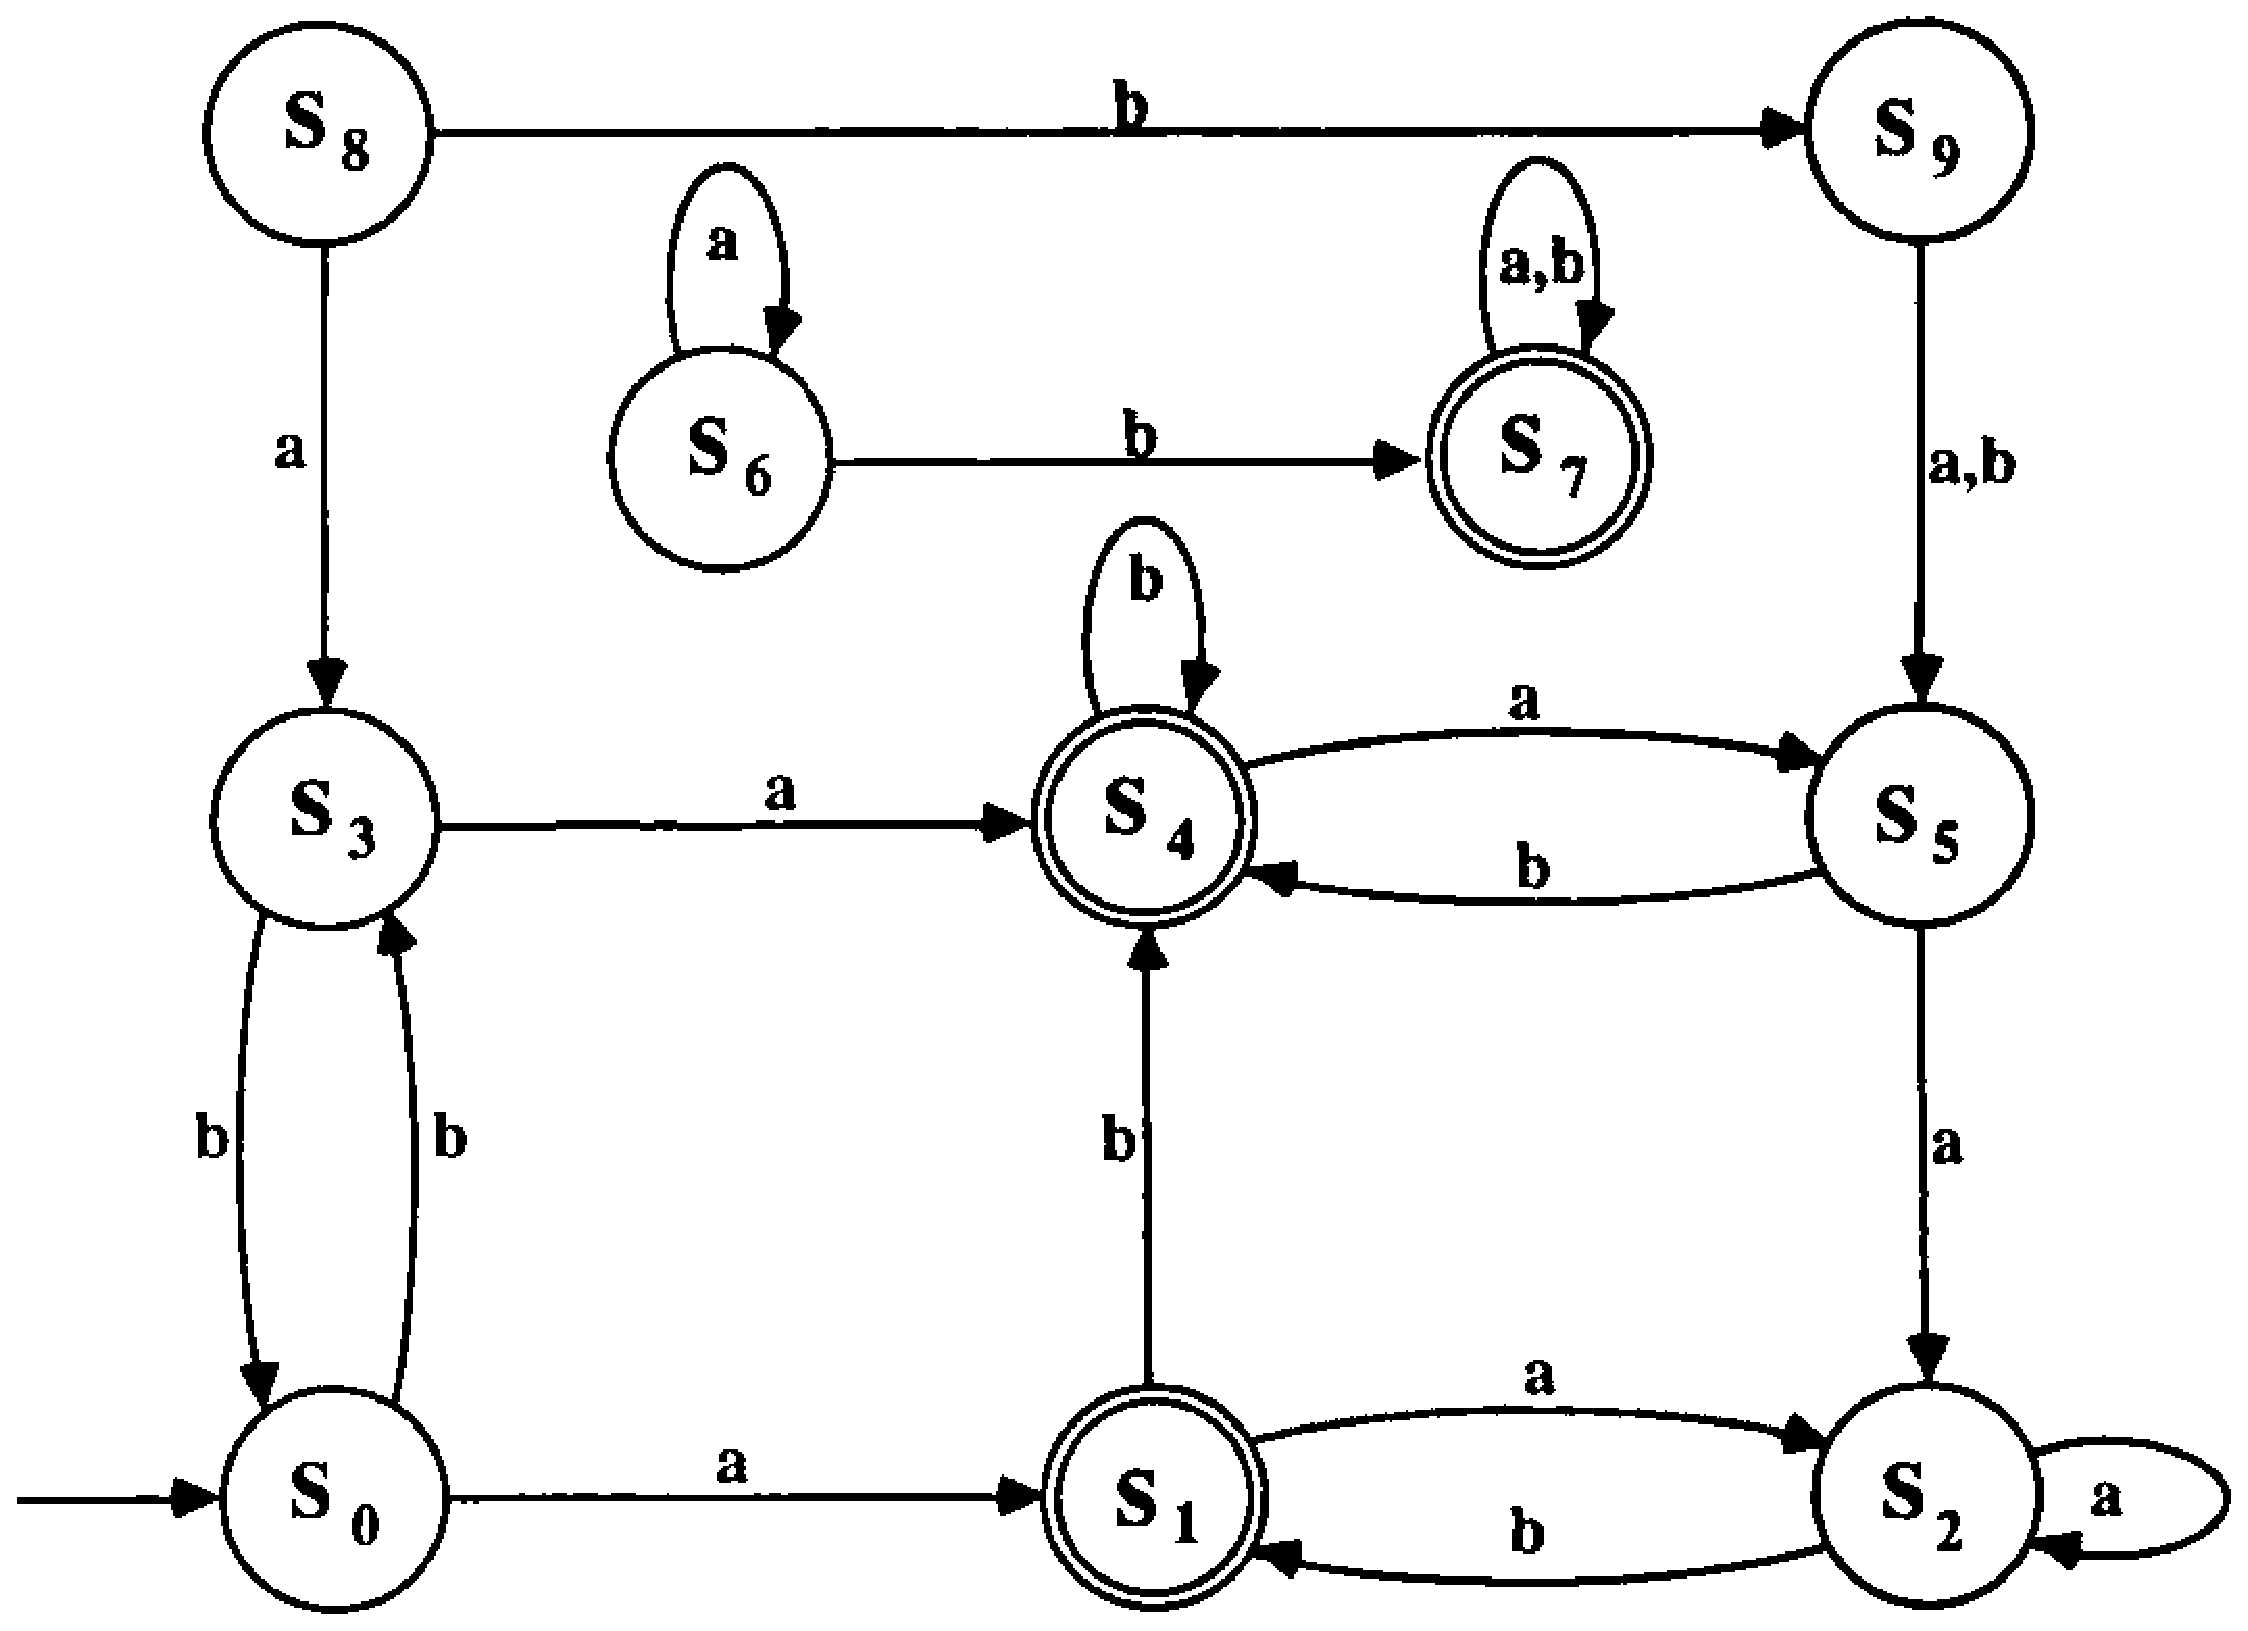
\epsfig{figure=ToFAfigures/fig3-9.eps,width=4.5in}}
\caption{The DFA D discussed in Example 3.15}\label{fig-3.9}
\end{figure}

The procedure for recursively calculating successive $C_i$s to determine $S^c$ provides
the final algorithm needed to efficiently find the minimal machine corresponding
to a given automaton $A$. From $A$, we use the $C_i$s to calculate $S^c$ and
thereby define $A^c$. Theorems \ref{thm-3.8} and related results suggest an
efficient algorithm for computing $E_A$ from which we can construct $A^c/_{E_{
A^c}}$. $A^c/_{E_{A^c}}$, is indeed the minimal machine equivalent to $A$, as
shown by the results in this chapter. Theorems \ref{thm-3.3} and \ref{thm-3.6}
show that $A^c/_{E_{A^c}}$ is equivalent to $A$. By Theorems \ref{thm-3.2},
\ref{thm-3.4}, and \ref{thm-3.5}, this automaton is reduced and connected, and
Corollary \ref{cor-3.4} guarantees that $A^c/_{E_{A^c}}$ must therefore be
minimal.

The proof of Theorem \ref{thm-3.7} suggests building a minimal equivalent deterministic
finite automaton for $A$ by first shrinking to a connected machine and then
reducing modulo the state equivalence relation, that is, by finding
$A^c/_{E_{A^c}}$. Theorem \ref{thm-3.5} assures us that when we reduce a connected machine
it will still be connected. An alternate strategy would be to first reduce
modulo $E_A$ and then shrink to a connected machine, that is, to find
$(A/_{E_A})^c$. In this case, we would want to make sure that connecting a
reduced machine will still leave us with a reduced machine. It can be shown that
if $A$ is reduced then $A^c$ is reduced (see the exercises), and hence this
method could also be used to find the minimal equivalent DFA.

Finding the minimal equivalent DFA by reducing $A$ first and then eliminating
the disconnected states is, however, less efficient than applying the algorithms
in the opposite order. Finding the connected set of states is simpler than
finding the state equivalence relation, so it is best to eliminate as many
states as possible by finding $S^c$ before embarking on the more complex search
for the state equivalence relation.

It should be clear that the algorithms in this chapter are presented in
sufficient detail to easily allow them to be programmed. As suggested in Chapter
\ref{ch-1}, the final states can be represented as a set and the transition function as a
matrix. The minimization procedures would then return the minimized matrix and
new final state set.

As a practical matter then, when generating an automaton to perform a given
task, our concern can be limited to defining a machine that \emph{works}. No further
creative insight is then necessary to find the minimal machine. Once a machine
that recognizes the desired language is found (however inefficient it may be),
the minimization algorithms can then be applied to produce a machine that is
both correct and efficient.

The proof that a reduced and connected machine is the most efficient was based
on the properties of the automaton $A_{R_L}$ obtained from the right congruence
$R_L$. This can be proved without relying on the existence of $A_{R_L}$. We
close this chapter with an outline of such a proof. The details are similar to
the proofs given in Chapter \ref{ch-7} for finite-state transducers.

Theorem \ref{thm-3.3}, which was not based in any way on $R_L$, implies that a minimal
DFA must be connected. Similarly, an immediate corollary of Theorem \ref{thm-3.6} is
that a minimal DFA must be reduced. Thus, a minimal machine is forced to be both
reduced and connected. We now must justify that a reduced and connected machine
is minimal. This result will follow from Corollary \ref{cor-3.3}, which can also be proved
without relying on $A_{R_L}$. The implication ($A \cong B \Rightarrow A$ is
equivalent to $B$) is due solely to the properties of isomorphisms and is
actually true irrespective of any other hypotheses (see the exercises).
Conversely, if $A$ is equivalent to $B$, then the fact that $A$ and $B$ are both
reduced and connected allows an isomorphism to be defined from $A$ to $B$ (see
the exercises).

Corollary \ref{cor-3.3} allows us to argue that any reduced and connected automaton $A$
is isomorphic to a minimal automaton $M$, and hence $A$ has as few states as $M$
and is minimal. The argument would proceed as follows: Since $M$ is minimal, we
already know that Theorems \ref{thm-3.3} and \ref{thm-3.6} imply that $M$ is reduced and connected.
Thus, $M$ and $A$ are two reduced and connected equivalent automata, and
Corollary \ref{cor-3.3} ensures that $A \cong M$. Thus, minimal machines are exactly those
that are reduced and connected.

\section*{Exercises}
\begin{enumerate}[{3.}1. ]
\item Use induction to show $(\forall s \in S)(\forall x \in \Sigma^*)
(\mu(\DBAR(s,x))=\DBAR_{R_L}(\mu(s), x))$ for the mapping $\mu$ defined in
Theorem \ref{thm-3.1}. %Do not appeal to the results of (5) in the proof of Theorem \ref{thm-3.1}.

\item Consider the state transition function given in Definition \ref{dfn-3.8} and use
induction to show
$$ (\forall x \in \Sigma^*)(\forall[s]_{E_A} \in S_{E_A})
	(\DBAR_{E_A}([s]_{E_A},x) = [\DBAR(s,x)]_{E_A}) $$

\item Prove that
$$ E_A = E_{0A} \cap E_{1A} \cap E_{2A} \cap E_{3A} \cap \cdots \cap E_{nA} \cap
	\cdots = \bigcap\limits^\infty_{j=0} E_{jA} $$

\item Given a finite automaton $A =\langle\Sigma,S,s_0,\delta,F\rangle$, show
that the function $\delta_{E_A}$ given in Definition \ref{dfn-3.8} is well defined.

\item Given a finite automaton $A =\langle\Sigma,S,s_0,\delta,F\rangle$, show
that the set $F_{E_A}$ given in Definition \ref{dfn-3.8} is a well-defined set.

\item Show that the range of the function $\delta^c$ given in Definition \ref{dfn-3.7} is
contained in $S^c$.

\item Prove Lemma \ref{lmm-3.1}.

\item Prove Lemma \ref{lmm-3.3}.

\item Prove Theorem \ref{thm-3.9}.

\item Given a homomorphism $\mu$ from the finite automaton 
$A=\langle\Sigma,S_A,s_{0A},\delta_A,F_A\rangle$ to the DFA 
$B=\langle\Sigma,S_B,s_{0B},\delta_B,F_B\rangle$, prove by induction that
$$ (\forall s \in S_A)(\forall x \in \Sigma^*)(\mu(\DBAR_A(s,x)) =
	\DBAR_B(\mu(s),x)) $$
	
\item Given a homomorphism $\mu$ from the finite automaton
$A=\langle\Sigma,S_A,s_{0A},\delta_A,F_A\rangle$ to the DFA 
$B=\langle\Sigma,S_B,s_{0B},\delta_B,F_B\rangle$, prove that $L(A)=L(B)$. As
long as it is explicitly cited, the result of Exercise 3.10 may be used without
proof.

\item \begin{enumerate}
\item Give an example of a DFA for which $A$ is \emph{not} connected and
$A/_{E_A}$ is not connected.
\item Give an example of a DFA for which $A$ is \emph{not} connected but
$A/_{E_A}$ \emph{is} connected.
\end{enumerate}

\item Given a finite automaton $A=\langle\Sigma,S,s_0,\delta,F\rangle$ and the
state equivalence relation $E_A$, show there exists a homomorphism from $A$ to
$A/_{E_A}$.

\item Given a \emph{connected} finite automaton
$A=\langle\Sigma,S,s_0,\delta,F\rangle$, show there exists a homomorphism from
$A$ to $A_{R_L}(A)$ by:
\begin{enumerate}
\item Define a mapping $\psi$ from $A$ to $A_{R_{L(A)}}$. (No justification need
be given.)
\item Prove that your $\psi$ is well defined.
\item Prove that $\psi$ is a homomorphism.
\end{enumerate}

\item Give an example to show that there may not exist a homomorphism from $A$
to $A_{R_{L(A)}}$ if $A$ is not connected (see Exercise 3.14).

\item Give an example to show that there may still exist a homomorphism from $A$
to $A_{R_{L(A)}}$ even if $A$ is not connected (see Exercise 3.14).

\item Give an example to show that, for the relations $R$ and $R_L$ given in
Theorem \ref{thm-2.2}, there need not exist a homomorphism from $A_{R_L}$ to $A_R$.

\item $\cong$ is an equivalence relation; in Chapter \ref{ch-2} we saw some equivalence relations
were also right congruences. Comment on the appropriateness of asking whether
$\cong$ is a right congruence.

\item Is $E_A$ a right congruence? Explain your answer.

\item Prove that if $A$ is reduced then $A^c$ is reduced.

\item For a homomorphism $\mu$ from $S_A$ to $S_B$ for the two finite automata
$A=\langle\Sigma,S_A,s_{0A},\delta_A,F_A\rangle$ and
$B=\langle\Sigma,S_B,s_{0B},\delta_B,F_B\rangle$,prove
$(\forall s,t \in S_A)(\mu(s) E_B \mu(t) \Leftrightarrow s E_A t)$.

\item Let $M$ be a DFA, and let $L=L(M)$.
\begin{enumerate}
\item Define an appropriate mapping $\psi$ from $M^c$ to $A_{(R^M)}$. (No justification need
be given.)
\item Prove that your $\psi$ is well defined.
\item Prove that $\psi$ is a homomorphism.
\item Prove that $\psi$ is a bijection.
\item Argue that $M^c \cong A_{(R^M)}$.
\end{enumerate}

\item For the machine $A$ given in Figure \ref{fig-3.10}a, find:
\begin{enumerate}
\item $E_A$ (list each $E_{iA}$)
\item $L(A)$
\item $A_{R_{L(A)}}$
\item $R_{L(A)}$
\item $A/_{E_A}$
\end{enumerate}

\item For the machine $B$ given in Figure \ref{fig-3.10}b, find:
\begin{enumerate}
\item $E_B$ (list each $E_{iB}$)
\item $L(B)$
\item $A_{R_{L(B)}}$
\item $R_{L(B)}$
\item $B/_{E_B}$
\end{enumerate}
Note that your answer to part (e) might contain some disconnected states.

\item For the machine $C$ given in Figure \ref{fig-3.10}c, find:
\begin{enumerate}
\item $E_C$ (list each $E_{iC}$)
\item $L(C)$
\item $A_{R_{L(C)}}$
\item $R_{L(C)}$
\item $C/_{E_C}$
\end{enumerate}
Note that your answer to part (e) might contain some disconnected states.

\item For the machine $D$ given in Figure \ref{fig-3.10}d, find:
\begin{enumerate}
\item $E_D$ (list each $E_{iD}$)
\item $L(D)$
\item $A_{R_{L(D)}}$
\item $R_{L(D)}$
\item $D/_{E_D}$
\end{enumerate}
Note that your answer to part (e) might contain some disconnected states.

% Figure 3.10
\begin{figure}
\centerline{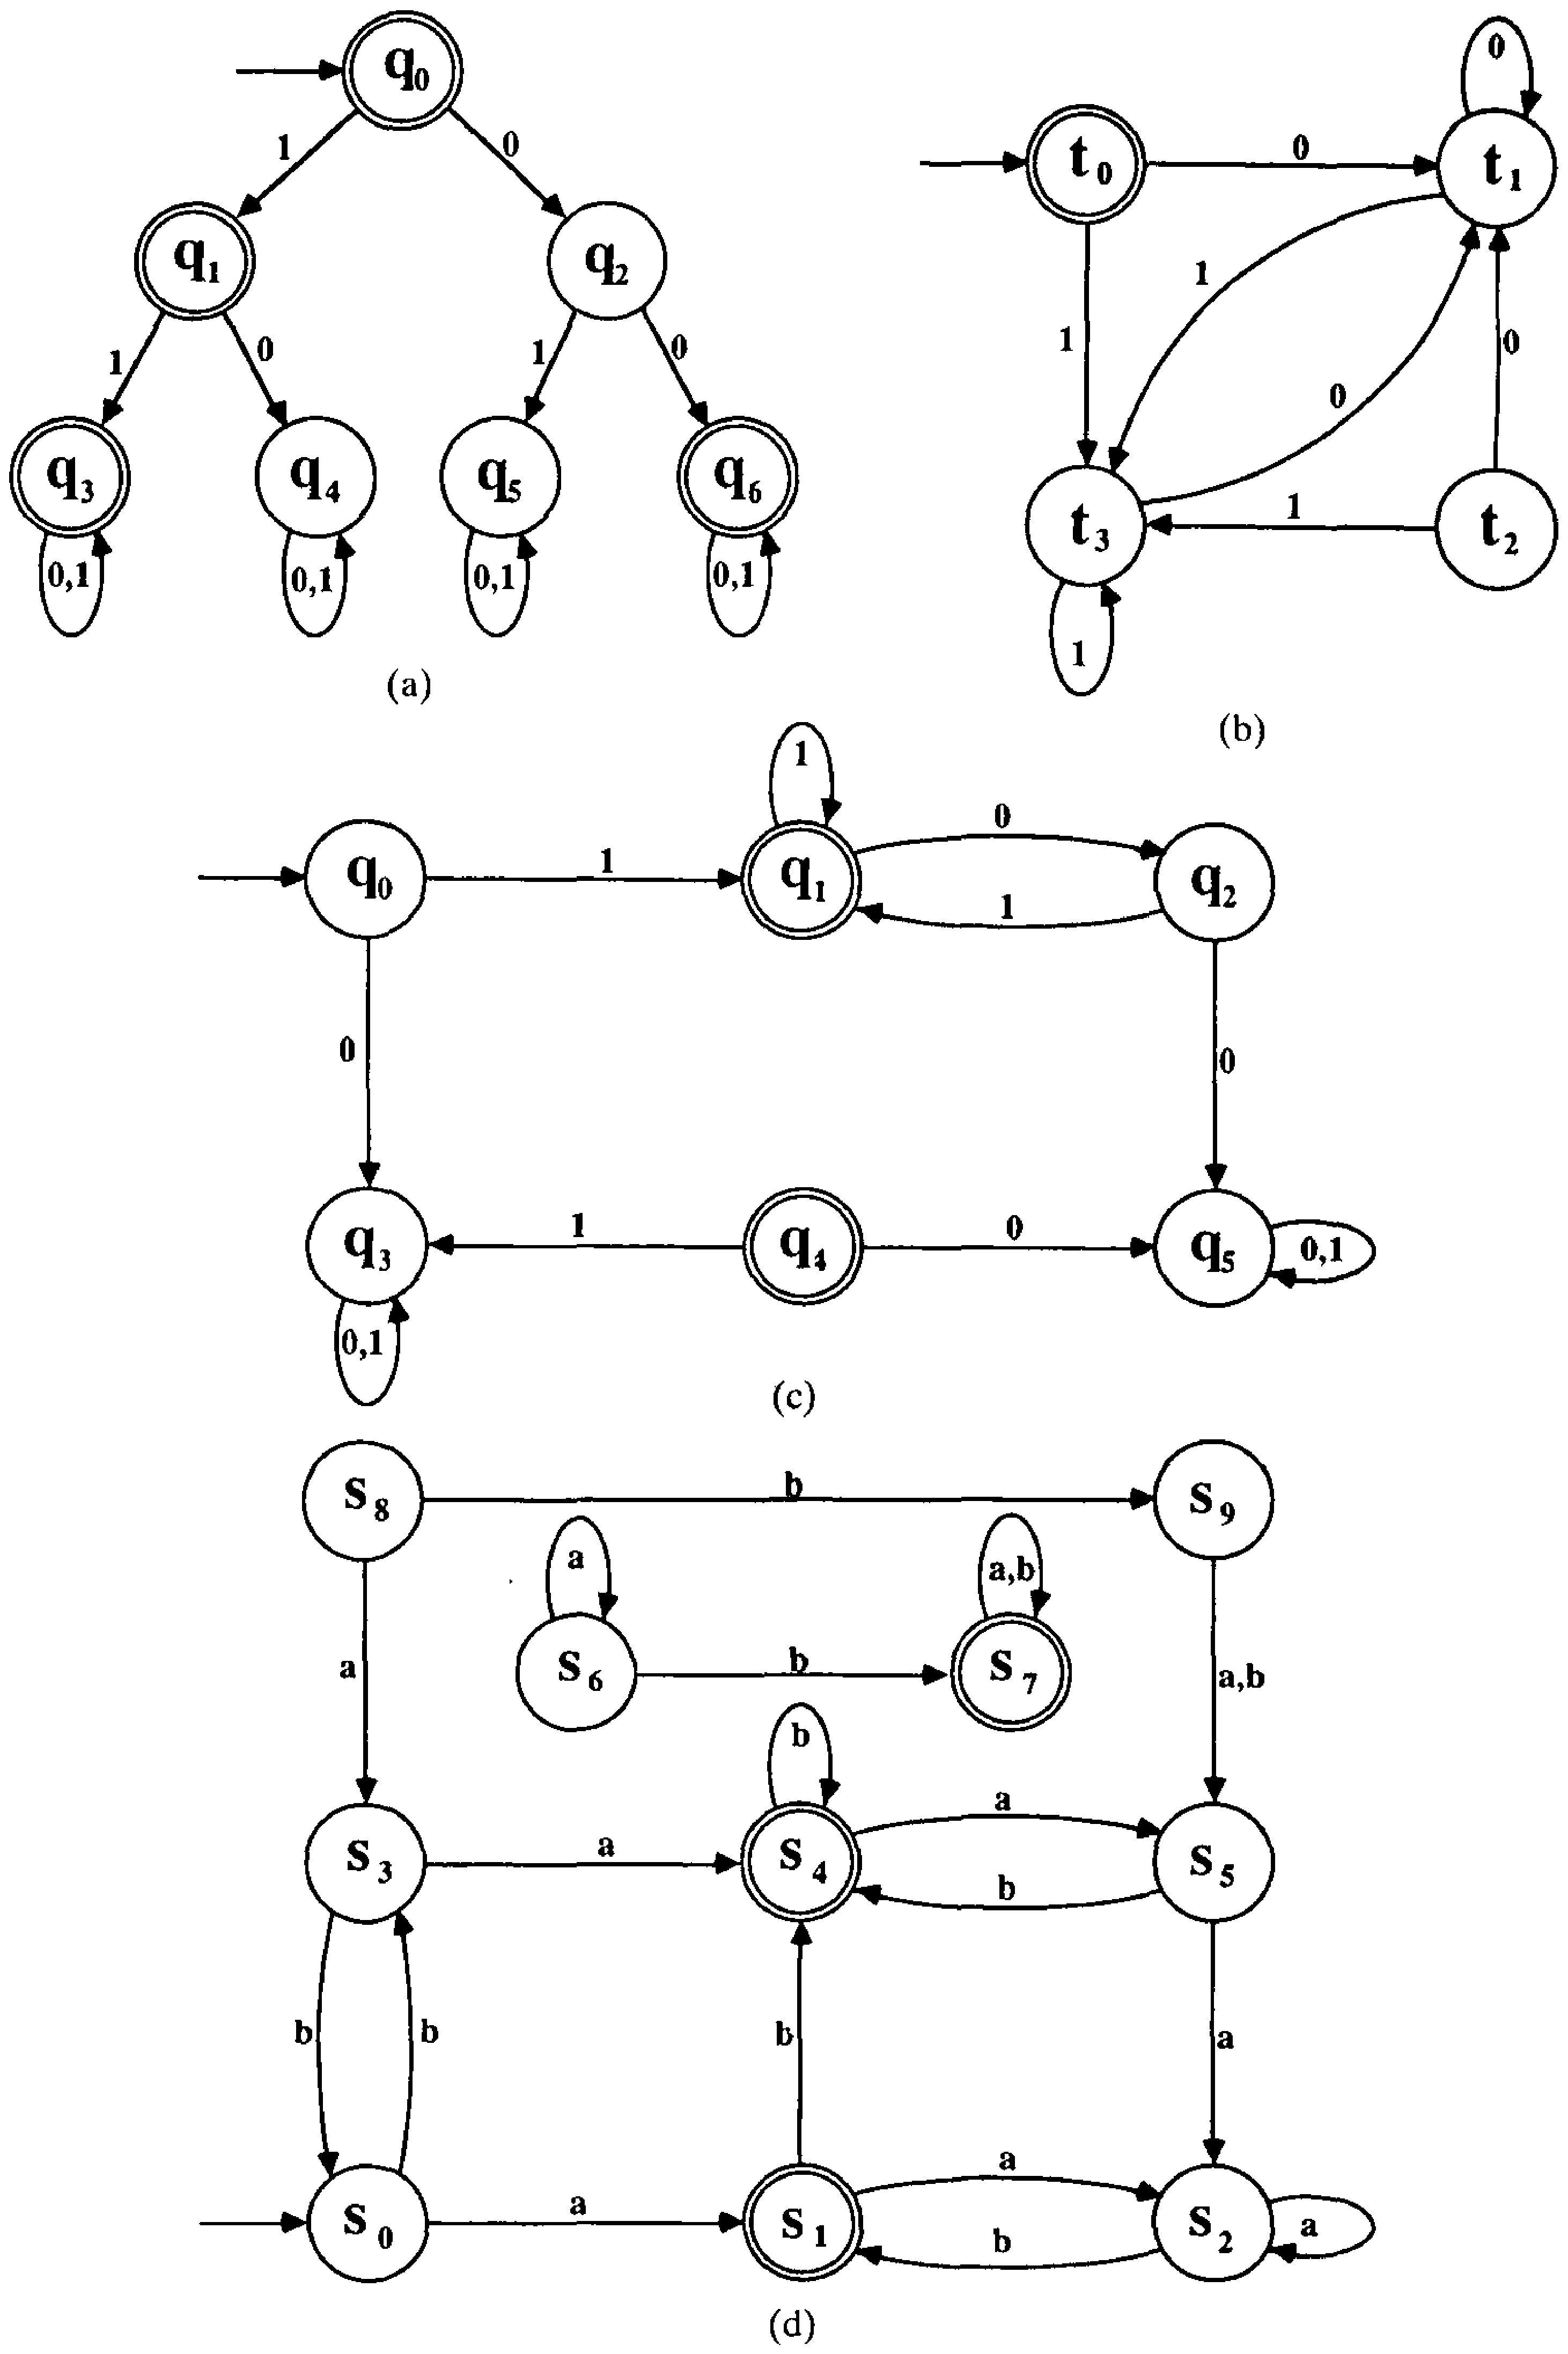
\epsfig{figure=ToFAfigures/fig3-10.eps,height=7.8in}}
\caption{(a) The DFA $A$ discussed in Exercise 3.23 (b) The DFA $B$ iscussed in
Exercise 3.24 (c) The DFA $C$ discussed in Exercise 3.25 (d) The DFA $D$
discussed in Exercise 3.26}\label{fig-3.10}
\end{figure}

\item Without relying on $A_{R_L}$, prove that if $A$ and $B$ are both reduced
and connected equivalent DFAs then $A \cong B$. Give the details for the
following steps: 
\begin{enumerate}
\item Define an appropriate function $\psi$ between the states of $A$ and the
states of $B$.
\item Show that $\psi$ is well defined.
\item Show that $\psi$ is a homomorphism.
\item Show that $\psi$ is a bijection.
\end{enumerate}

\item In the proof of (6) in Theorem \ref{thm-3.1}, the transition from line 3 to line 4 only involved
$\Rightarrow$ rather than $\Leftrightarrow$. Show by means of an example that
the two expressions involved in this transition are not equivalent.

\item Supply reasons for each of the equivalences in the proof of Theorem \ref{thm-3.8}.

\item Minimize the machine defined in Figure \ref{fig-3.3}.

\item \begin{enumerate}
\item Give an example of a DFA for which $A$ is \emph{not} reduced and $A^c$ is
not reduced.
\item Give an example of a DFA for which $A$ is \emph{not} reduced and $A^c$
\emph{is} reduced.
\end{enumerate}

\item Note that $\cong$ relates some automata to other automata, and therefore
$\cong$ is a relation over the set of all deterministic finite automata.
\begin{enumerate}
\item For automata $A,\ B$, and $C$, show that if $g$ is an isomorphism from $A$
to $B$ and $f$ is an isomorphism from $B$ to $C$, then $f \circ g$ is an
isomorphism from $A$ to $C$.
\item Prove that $\cong$ is a symmetric relation; that is, formally justify that
if there is an isomorphism from $A$ to $B$ then there is an isomorphism from $B$
to $A$.
\item Prove that $\cong$ is a reflexive relation.
\item From the results in parts (a), (b), and (c), prove that $\cong$ is an
equivalence relation over the set of all deterministic finite automata.
\end{enumerate}

\item Show that homomorphism is \emph{not} an equivalence relation over the set of
all deterministic finite automata.

\item For the relations $R$ and $R_L$ given in Theorem \ref{thm-2.2}, show that there
exists a homomorphism from $A_R$ to $A_{R_L}$.

\item Prove that if there is a homomorphism from $A$ to $B$ then $R^A$ refines
$R^B$.

\item Prove that if $A$ is isomorphic to $B$ then $R^A=R^B$
\begin{enumerate}
\item By appealing to Exercise 3.35.
\item Without appealing to Exercise 3.35.
\end{enumerate}

\item Consider two deterministic finite automata for which $A$ is not
homomorphic to $B$, but $R^A=R^B$.
\begin{enumerate}
\item Give an example of such automata for which $L(A) = L(B)$.
\item Give an example of such automata for which $L(A) \not= L(B)$.
\item Can such examples be found if both $A$ and $B$ are connected and
$L(A)=L(B)$?
\item Can such examples be found if both $A$ and $B$ are reduced and
$L(A)=L(B)$?
\end{enumerate}

\item Disprove that if $A$ is homomorphic to $B$ then $R^A=R^B$.

\item Prove or give a counterexample [assume $L = L(M)$].
\begin{enumerate}
\item For any DFA $M$, there exists a homomorphism $\psi$ from $A_{(R^M)}$ to
$M$.
\item For any DFA $M$, there exists an isomorphism $\psi$ from $A_{(R^M)}$ to
$M$.
\item For any DFA $M$, there exists a homomorphism $\psi$ from $M$ to
$A_{(R^M)}$.
\end{enumerate}

\item Prove that if $A$ is a minimal DFA then $R^A = R_{L(A)}$.

\item Give an example to show that Exercise 3.40 can be false if $A$ is not
minimal.

\item Give an example to show that Exercise 3.40 may still hold if $A$ is not
minimal.

\item Definition \ref{dfn-3.8} takes an equivalence relation of the set of states $S$ and
defines a machine based on that relation. In general, we could choose a relation
$R$ in $S$ and define a machine $A/_R$ (as we did when we defined $A/_{E_A}$
when the relation $R$ was $E_A$).
\begin{enumerate}
\item Consider $R=E_{0A}$. Is $A/_{E_{0A}}$ always well defined? Give an example
to illustrate your answer.
\item Assume $R$ is a refinement of $E_A$. Is $A/_R$ always well defined? For
the cases where it is well defined, consider the theorems that would correspond
to Theorems \ref{thm-3.4}, \ref{thm-3.5}, and \ref{thm-3.6} if $E_A$ were replaced by such a refinement $R$.
Which of these theorems would still be true?
\end{enumerate}

\item Given a DFA $M$, prove or give a counterexample.
\begin{enumerate}
\item There exists a homomorphism from $M/_{E_M}$ to $A_{R_{L(M)}}$.
\item There exists a homomorphism from $A_{R_{L(M)}}$ to $M/_{E_M}$.
\end{enumerate}

\item Prove that the bound given for Theorem \ref{thm-3.11} can be sharpened: given a
finite automaton $A=\langle\Sigma,S,s_0,\delta,F\rangle$,
$(\exists m \in \NN \ni m < \|S\| \wedge E_{mA} = E_{m+1A})$.

\item Prove or give a counterexample:
\begin{enumerate}
\item If $A$ and $B$ are equivalent, then $A$ and $B$ are isomorphic.
\item If $A$ and $B$ are isomorphic, then $A$ and $B$ are equivalent.
\end{enumerate}

\item Given a finite automaton $A =\langle\Sigma,S,s_0,\delta,F\rangle$, prove
that the $C_i$s given in Definition \ref{dfn-3.10} are nested:
$(\forall i \in \NN)(C_i \subseteq C_{i+1})$.

\item Prove (by induction) that $C_i$ does indeed represent the set of all
states that can be reached from $s_0$ by strings of length $i$ or less.

\item Prove that, given a finite automaton
$A =\langle\Sigma,S,s_0,\delta,F\rangle$,
$$ (\exists i \in \NN \ni C_i=C_{i+1}) \Rightarrow
	(\forall k \in \NN)(C_i = C_{i+k}). $$

\item Prove that, given a DFA $A =\langle\Sigma,S,s_0,\delta,F\rangle$,
$(\exists i \in \NN \ni C_i = C_{i+1}) \Rightarrow (C_i = S^c)$.

\item Prove that, given a finite automaton
$A =\langle\Sigma,S,s_0,\delta,F\rangle,\ \exists i \in \NN \ni C_i = C_{i+1}$.

\item Prove that, given a DFA $A =\langle\Sigma,S,s_0,\delta,F\rangle$,
$(\exists i \in \NN \ni i \leq \|S\| \wedge C_i = S^c)$.

\item Use the results of Exercises 3.47 through 3.52 to argue that the procedure
for generating $S^c$ from successive calculations of $C_i$ is correct and is
actually an algorithm.

\item Give an example of two DFAs $A$ and $B$ that simultaneously satisfy the
following three criteria:
\begin{enumerate}[1.]
\item There is a homomorphism from $A$ to $B$.
\item There is a homomorphism from $B$ to $A$.
\item There does not exist any isomorphism between $A$ and $B$.
\end{enumerate}

\item Assume $R$ and $Q$ are both right congruences of finite rank, $R$ refines
$Q$, and $L$ is a union of equivalence classes of $Q$.
\begin{enumerate}
\item Show that $L$ is also a union of equivalence classes of $R$.
\item Show that there exists a homomorphism from $A_R$ to $A_Q$. (\emph{Hint:}
Do \emph{not} use the $\mu$ given in Theorem \ref{thm-3.1}; there is a far more
straightforward way to define a mapping.)
\item Give an example to show that there need not be a homomorphism from $A_Q$
to $A_R$.
\end{enumerate}

\item Prove that $A_Q$ must be connected.

\item Prove that if there is an isomorphism from $A$ to $B$ and $A$ is connected
then $B$ must also be connected.

\item Prove that if there is an isomorphism from $A$ to $B$ and $B$ is connected
then $A$ must also be connected.

\item Disprove that if there is a homomorphism from $A$ to $B$ and $A$ is
connected then $B$ must also be connected.

\item Disprove that if there is a homomorphism from $A$ to $B$ and $B$ is
connected then $A$ must also be connected.

\item Given a DFA $A$, recall the relation $R^A$ on $\Sigma^*$ induced by $A$.
This relation gives rise to another DFA $A_{(R^A)}$ [with $Q=R^A$ and $L=L(A)$].
Consider also the connected version of $A$, $A^c$.
\begin{enumerate}
\item Define an isomorphism $\psi$ from $A_{(R^A)}$ to $A^c$. (No justification
need be given.)
\item Prove that your $\psi$ is well defined.
\item Prove that $\psi$ is a homomorphism.
\item Prove that $\psi$ is an isomorphism.
\end{enumerate}

\item Assume that $A$ and $B$ are connected DFAs. Assume that there exists an
isomorphism $\psi$ from $A$ to $B$ and an isomorphism $\mu$ from $B$ to $A$.
Prove that $\psi = \mu^{-1}$.

\item Assume that $A$ and $B$ are DFAs. Assume that there exists an isomorphism
$\psi$ from $A$ to $B$ and an isomorphism $\mu$ from $B$ to $A$. Give an example
for which $\psi \not= \mu^{-1}$.

\item Give an example of a three-state DFA for which $E_{0A}$ has only one
equivalence class. Is it possible for $E_{0A}$ to be different from $E_{1A}$ in
such a machine? Explain.

\item Assume A and B are both reduced and connected. If $\psi$ is a homomorphism
from $A$ to $B$, does $\psi$ have to be an isomorphism? Justify your
conclusions.

\item Prove Corollary \ref{cor-3.2}.

\item Prove that $S^c =\{\DBAR(s_0,x)|\ |x| \leq \|S\|\}$.

\item Given a finite automaton $A=\langle\Sigma,S,s_0,\delta,F\rangle$, two
states $s,t \in S$, and the automata $A^t=\langle\Sigma,S,t,\delta,F\rangle$ and
$A^s=\langle\Sigma,S,s,\delta,F\rangle$, prove that $s E_A t \Leftrightarrow
L(A^s) = L(A^t)$.

\item Given a finite automaton $A=\langle\Sigma,S,s_0,\delta,F\rangle$, consider
the terminal sets $T(A,t)=\{x$ $|$ $\DBAR(t,x) \in F\}$ and initial sets
$I(A,t)=\{x$ $|$ $\DBAR(s_0,x) = t\}$ for each $t \in S$.
\begin{enumerate}
\item Prove that the initial sets of $A$ must form a partition of $\Sigma^*$.
\item Give an example to show that the terminal sets of $A$ might not partition
$\Sigma^*$.
\item Give an example to show that the terminal sets of $A$ might partition
$\Sigma^*$.
\end{enumerate}
\end{enumerate}
